% 国赛 (CUMCM) 2026 兼容模板
% 基于社区维护的 latexstudio/CUMCMThesis，并以全国组委会 2026 格式规范为准。
% cumcmthesis 不是组委会指定的唯一 TeX 模板。
% 电子版提交使用 withoutpreface 去掉封面编号页，bwprint 黑白打印
\documentclass[withoutpreface,bwprint]{cumcmthesis}

% === 额外宏包（cumcmthesis 已内置 amsmath/graphicx/booktabs/listings/hyperref/tabularx/longtable 等）===
\usepackage[framemethod=TikZ]{mdframed}
\usepackage[section]{placeins}
\usepackage{needspace}
\usepackage{algorithm2e}

% === 参考文献引用（数字型，配合 gbt7714-numerical.bst）===
%  不要加载 cite 宏包 — 它与 natbib 冲突会导致编译错误。
%  必须显式加载 natbib：gbt7714-numerical.bst 产出的是 natbib 风格条目
%    （\bibitem[作者(年)]{key}），不加载 natbib 时标准 \cite 会把“作者-年”当引用标记
%    上标出来（而非数字 [1]）。numbers 模式让 \cite 产出数字，cls 的 \upcite 再上标它。
%    正文引用统一用 \upcite{key} 得数字上标 $^{[1]}$。
\usepackage[numbers,sort&compress]{natbib}

% === TikZ（cumcmthesis 已加载 tikz，这里只加额外库）===
\usetikzlibrary{arrows.meta,positioning,shapes.geometric,fit,calc}

% === 代码高亮设置 ===
\lstset{
    language=Python,
    basicstyle=\small\ttfamily,
    breaklines=true,
    frame=single,
    numbers=left,
    numberstyle=\tiny,
}

% === 摘要后排版修复 ===
%  不再重定义 \@cite —— 引用交给 natbib（上面已 numbers 模式加载），
%    \upcite 会正确产出数字上标；旧的 \@cite hack 在 natbib 下无效且会干扰，已移除。
\makeatletter
% === 修复摘要后排版（cls 的 abstract 结束时有 \newpage\null，可能产生空白页）===
% 方案：abstract 结束时只换页，不加 \null；正文不生成目录。
\renewenvironment{abstract}{%
  \if@twocolumn\section*{\abstractname}%
  \else\begin{center}{\zihao{3}\bfseries \abstractname\vspace{-.5em}\vspace{\z@}}\end{center}\quotation
  \fi}{\if@twocolumn\else\endquotation\newpage\fi}
\makeatother

% === 竞赛信息（电子版提交时注释掉）===
% \tihao{A}
% \baominghao{xxxx}
% \schoolname{[学校名称]}
% \membera{[成员A]}
% \memberb{[成员B]}
% \memberc{[成员C]}
% \supervisor{[指导老师]}
% \yearinput{[竞赛年份]}
% \monthinput{[月]}
% \dayinput{[日]}

\title{药材热风烘干的热质耦合输运模型与烘干时长预测}

% MH-FLOAT-TUNE 受控浮动调参（防整页空白/一页一图）
% placeins 已由模板/cls 加载，此处不重复注入（避免 Option clash）
\renewcommand{\topfraction}{0.92}
\renewcommand{\bottomfraction}{0.9}
\renewcommand{\textfraction}{0.06}
\renewcommand{\floatpagefraction}{0.72}
\renewcommand{\dbltopfraction}{0.92}
\renewcommand{\dblfloatpagefraction}{0.72}
\setcounter{topnumber}{3}
\setcounter{bottomnumber}{2}
\setcounter{totalnumber}{4}
% 正文使用自然页底；避免强制齐底造成的无信息留白。
\raggedbottom
\begin{document}

\maketitle

% === 摘要 ===
\begin{abstract}

药材内部的温度与含水率无法实测，可调的工艺量只有送风温度与含湿量，
故需用数学模型代替逐一试烘。

针对问题一，建立一维轴对称热-质耦合输运模型：两场均以第三类边界条件与热风
耦合，传质驱动力直接取空气含湿量，避免自拟题设之外的吸附等温线。空间上采用
\textbf{节点中心有限体积}格式使表面 Robin 条件以原始形式进入方程组，
时间上用后向 Euler
格式配合 Picard 迭代。热 Biot 数 $1.3889$ 表明内外热阻相当。温度方程在常物性
下线性且与水分方程解耦，据此推导减法形式的\textbf{Bessel--Duhamel 解析解}
作独立校验，最大偏差仅 $5.224\times10^{-4}$ °C。$1800$ s 时中心温度
$33.5757$ °C、表面 $36.7857$ °C；中心含水率仍为 $2.5500$ kg/kg、表面已降到
$1.5103$ kg/kg，预热段仅排出初始水分的 $10.06\%$。

针对问题二，物性全程统一采用附录 3，其扩散系数含 Arrhenius 因子，温度由
$28$ °C 升到 $50$ °C 使之增大为原来的 $2.39$ 倍。$3$ h 时中心含水率降到
$\mathbf{1.7662}$ kg/kg，同期内外温差由 $0.5$ h 的 $3.2235$ °C 收缩到
$0.1169$ °C，说明该时窗内\textbf{热已基本平衡而质仍在进行}；
由此判断后两问的烘干时长主要由传质控制，温度的作用主要经扩散系数传递。

针对问题三，把“各处水分浓度低于 $0.15$ kg/kg”定义为作用在空间最大值上的
\textbf{逐点首达判据}。程序按全域最大值判定；各算例的含水率剖面均沿半径单调
递减，故该场判据与中心判据给出同一时刻。按相邻输出步线性插值求得烘干时长
$\mathbf{57.4247}$ h，
即 $2.3927$ d，落在题面所给 $2$ 至 $3$ 天区间内，全程离散守恒残差
$3.425\times10^{-10}$。若误用截面平均判据则得约 $36$ h，短 $37\%$，
而该时刻中心仍有 $0.1858$ kg/kg 未达标。

针对问题四，为处理收缩动边界，定义\textbf{干质量拉格朗日坐标}
$s=(r/R(t))^2$，把收缩降格为方程与表面通量中两个已知的标量系数，
既不产生伪对流项，也消去柱坐标在轴心的奇点，四问由此共用同一求解器。
取附录 4 物性并按附件 2 令
半径由 $2.000$ cm 收缩（全程最小 $1.198$ cm，$35$ h 后已冻结在 $1.200$ cm），
求得 $\mathbf{51.0711}$ h，
即 $2.1280$ d，较定域情形仅短 $11.0\%$。通过 $2\times2$ 消融实验把这一净变化
拆为物性效应 $+126.0\%$、收缩效应 $-56.1\%$ 与\textbf{交互项 $-46.5145$ h}，
说明两机制不可线性叠加，收缩才是最强的单一因素；灵敏度排序
$R\gg h_m>T_{\mathrm{air}}\gg W_{\mathrm{air}}\gg h$ 与半径弹性 $1.810$
与这一判断一致。

\keywords{热质耦合输运\quad 干质量拉格朗日坐标\quad 节点中心有限体积\quad
阈值首达时刻\quad 消融实验}
\end{abstract}

% === 摘要与正文之间的换页 ===
%  不要在这里加回 \tableofcontents：竞赛论文统一不出目录页。
% abstract 环境结尾已经换页；这里不再重复 \clearpage，避免空白页边缘情况。

% === 正文 ===
% 这两个标签只供编译合规检查精确计算 CUMCM 正文页数，不显示在论文中。
\label{mh:body-start}
\section{问题背景与问题重述}

热风烘干是中药材产地初加工中最常见的干燥方式，通常包含预热平衡与恒温干燥两个
阶段：先把冷料升温到接近热风温度，再在温湿度基本恒定的环境中持续排出水分。
烘房的送风温度与送风含湿量是唯一可直接调控的工艺量，而药材内部的温度与含水率
并不能实时测量。工艺参数选得不合适，干燥效率、能耗与成品品质会同时受损；
逐一试烘的代价又很高。因此需要建立能刻画药材内部温度场与含水率场演化的
数学模型，用数值仿真代替试验，回答“内部什么时候热透”“什么时候各处都达标干燥”
这两类问题\upcite{khallaf2022herbs,le2025acori}。

\subsection{题设条件}

待烘药材形状近似圆柱，长 $25$ cm、半径 $2$ cm。烘干开始时药材温度为 $28$ °C，
水分浓度（即干基含水率，指每千克绝干物料所含水的千克数）为 $2.55$ kg/kg，
两者在药材内部均匀分布。附件 1 给出烘房热风的温度（单位 °C）与水分浓度
（即空气含湿量，单位 kg/kg）从 $0$ 到 $14400$ s 每 $60$ s 一个点的实测时程。
附件 2 给出烘干过程中各时间点药材的半径（单位 cm），时间跨度 $0$ 至 $259200$ s、
间隔 $1800$ s。附录 2 给出预热平衡阶段所需的密度、比热容、热传导系数、
对流换热系数、对流传质系数与水分扩散系数；附录 3 与附录 4 分别给出另外两套
随含水率与温度变化的物性经验公式。整个烘干过程一般持续 $2$ 至 $3$ 天，
按烘干要求，药材各处的水分浓度应低于 $0.15$ kg/kg。全部结果保留四位小数。

\subsection{待求问题}

\textbf{问题一}　建立预热平衡阶段药材温度和水分浓度变化规律的数学模型，
相关参数取附录 2。给出 $100$、$300$、$600$、$900$、$1200$、$1500$、$1800$ s
七个时刻，到药材中心距离 $0$、$0.5$、$1$、$1.5$、$2$ cm 五个位置处的温度与
水分浓度，并另行提交 $1800$ s 内每隔 $1$ s、到药材中心距离每隔 $0.1$ cm 的
完整结果。

\textbf{问题二}　建立整个烘干过程药材温度和水分浓度变化规律的数学模型，
经验公式统一采用附录 3。给出 $3$ h 内每隔 $0.5$ h、上述五个位置处的温度与
水分浓度，并另行提交每隔 $1$ s、每隔 $0.1$ cm 的完整结果。

\textbf{问题三}　在药材各处水分浓度均低于 $0.15$ kg/kg 的烘干要求下，
确定烘干所需要的时间（单位 h）。给出每隔 $6$ h、到药材中心距离每隔 $0.5$ cm
的水分浓度，末行为烘干结束时刻，并另行提交每隔 $60$ s、每隔 $0.1$ cm 的
完整结果。

\textbf{问题四}　考虑药材因水分流失发生的尺寸变化，根据附件 2 确定烘干时长，
经验公式见附录 4。给出每隔 $6$ h、每隔 $0.5$ cm 的水分浓度，末列为药材表面处的
数值，末行为烘干结束时刻，并另行提交每隔 $60$ s、每隔 $0.1$ cm 的完整结果。

\section{问题分析}

四问要求的输出各不相同（两问要场分布、两问要时长），但支配现象的物理机制只有
一套：热量由热风经表面传入药材并向内部扩散，水分由内部扩散到表面后被气流带走。
因此本文先建立一个统一的一维轴对称耦合输运模型，再按各问指定的物性闭合与几何
条件逐层放开，四问共用同一份控制方程与同一套离散格式。图~\ref{fig:problem_relation}
给出四问的依赖关系：横向看是物性闭合从常物性到两套变物性的更替，纵向看是求解
诉求从给定时窗的场分布升级为阈值首达时刻，最后叠加求解域自身的收缩。

\begin{figure}[!htbp]
  \centering
  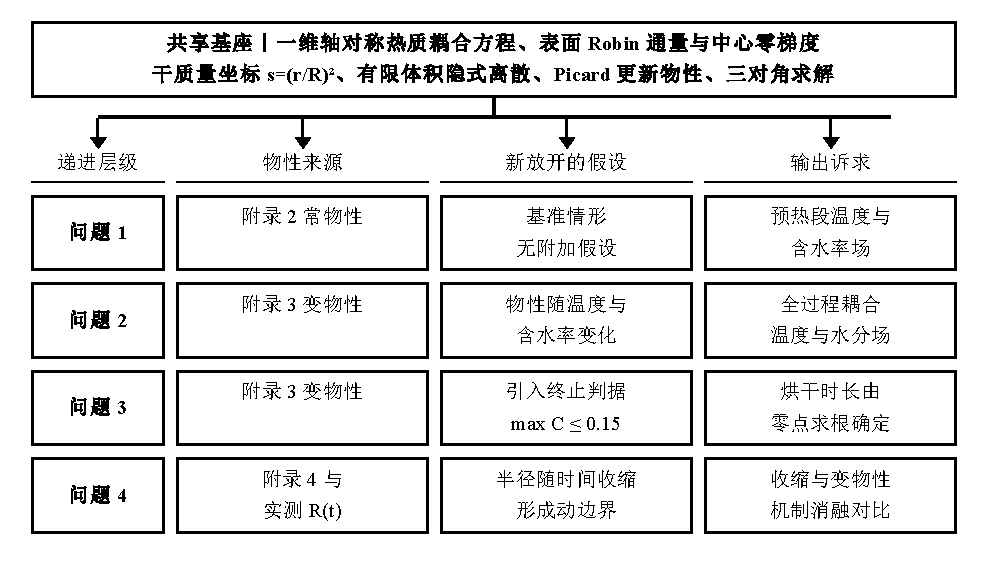
\includegraphics[width=0.9\textwidth,height=0.8\textheight,keepaspectratio]{../figures/fig_problem_relation_drawio.pdf}
  \caption{四问关系与递进层次}
  \label{fig:problem_relation}
\end{figure}

这一结构也决定了后文的写法：第~\ref{sec:model}~节把四问共用的守恒关系、
坐标变换与离散格式集中推导一次，此后每一问只交代它保留了什么、新增了什么、
结果因此改变了什么，不再重复整套方程。

\subsection{问题一的分析}

问题一要的是预热平衡阶段的两个场。判断模型维数不能只看几何：$L/R=12.5$ 说明
侧面传递远比端面重要，而题目要求的输出只按“到药材中心的距离”一个坐标索引——
若保留轴向坐标，同一半径不同高度处的温度并不相同，制表就没有唯一答案。
两条证据同时指向一维径向轴对称。

附录 2 的密度、比热容与热传导系数都是常数，只有水分扩散系数依赖含水率。
温度方程因此是线性的，可以用 Bessel 特征函数展开配合 Duhamel 叠加求出解析解；
含水率方程仍是非线性的，只能数值求解。这给出了一条难得的独立校验通道：
用解析解检验数值求解器在温度场上的正确性，再把同一套离散格式用于含水率场，
从而把“程序实现是否正确”与“物理建模是否恰当”分开验证。

表面换热强度需要先估计。热 Biot 数 $hR/k=1.3889$ 处于内外热阻相当的区间，
既不能把药材当作温度均匀的集中参数体，也不能把表面温度直接钉在热风温度上，
必须解偏微分方程并采用第三类边界条件。传质一侧的量级更悬殊：初始含水率下
扩散系数约 $4.94\times10^{-9}$ m$^2$/s，对应的质 Biot 数约 $3.24$。
两个方向的阻力都不可忽略。

一个需要提前判定的取舍是汽化潜热。附录未给出汽化潜热数值，若在温度边界条件中
补入蒸发冷却项并按常见量级 $2.4\times10^6$ J/kg 估算，$1800$ s 时蒸发耗热约
$655$ W/m$^2$，而同期对流供热仅约 $118$ W/m$^2$，净热流为负、药材应当降温，
与附件 1 给出的升温工况和“预热”这一名称直接矛盾。故本题的既定语义是热、
质两个通道分别按对流规律传递，不引入潜热耦合项。

\subsection{问题二的分析}

问题二把时间窗从预热段拉长到整个烘干过程，并明确要求经验公式统一采用附录 3。
“统一”二字排除了按阶段切换物性的做法：即使在 $t\le1800$ s 的预热段，
也应使用附录 3 而非附录 2。由此产生一个必须显式说明的现象——问题二在
$1800$ s 处给出的数值与问题一并不相同。这不是前后矛盾，而是两问采用了不同的
物性闭合，若不说明，容易被误读为计算不自洽。

附录 3 只重新给出了密度、比热容、热传导系数与扩散系数，没有重新给出对流换热
系数与对流传质系数，故这两个表面系数沿用附录 2 的取值，这是不引入任何自由参数的
唯一读法。附录 3 的三个物性都写成湿基含水率 $C/(C+1)$ 的线性函数，
初始状态下该组合等于 $0.7183$；若误把它简化为干基含水率 $C$，热传导系数会被
放大两倍以上。扩散系数中的 $\mathrm{e}^{-3850/T}$ 属于 Arrhenius 型，
指数上的 $3850$ 已经含有活化能与气体常数之比，温度必须用热力学温标；
误用摄氏温标会使扩散系数偏离数十个数量级。

附件 1 只覆盖到 $14400$ s，而全过程需要几十小时，故必须约定此后的烘房条件。
附件 1 末段已进入平台，采用末 $24$ 个数据点的均值作为恒温干燥段的取值既符合
“恒温干燥”的字面含义，也有数据支撑，且比取单点更能抑制测量波动。
这一约定支配了后两问绝大部分时间轴，其影响必须与结果一同披露。

\subsection{问题三的分析}

问题三新增的内容只有终止判据。“各处的水分浓度应低于 $0.15$ kg/kg”是一个
作用在空间最大值上的条件，而不是作用在截面平均值上的条件。这一区分在本题
量级很大：本文实际算得的平均含水率在 $36$ h 就已降到 $0.1499$，若误用均值判据
会得到约 $36$ h 的答案，比逐点判据短三成以上，而此时中心处仍有 $0.1858$ kg/kg，
药材内部远未达标。

含水率剖面沿半径单调递减这一性质使空间最大值取于中心，于是场判据可化为
一个标量判据，阈值首达时刻用相邻输出步之间的插值定位。判据能否在有限时间内达到也需要
检验：表面处的驱动浓度由空气含湿量给出，其平台值约 $0.05$ kg/kg，低于阈值
$0.15$ kg/kg，故存在有限的达标时刻。题面“一般持续 $2$ 至 $3$ 天”给出了一个
独立于模型之外的量级区间，可用来反查答案是否落在合理范围。

\subsection{问题四的分析}

问题四相对问题三只增加两件事：物性闭合换成附录 4，半径由固定值改为附件 2 给出的
实测时程。“请根据附件 2”意味着收缩是给定的运动学数据，不是待求量，
因此模型不需要补充任何收缩本构，也不应由含水率反推半径。附件 2 显示半径从
$2.000$ cm 单调降到 $1.198$ cm，横截面积仅剩三分之一略多，而全部收缩量的
$78.1\%$ 发生在前 $6$ h，正是传质最活跃的时段，扩散路程在最关键的阶段被大幅缩短。

两个新增因素的作用方向相反：附录 4 在初始状态下给出的扩散系数比附录 3 小 $5.4$ 倍，
使干燥变慢；收缩缩短扩散路程，使干燥变快。若只比较问题三与问题四的总时长，
净变化不大，很容易得出“收缩影响有限”的错误判断。因此必须做四组合的消融实验，
把两个机制分别量化，再检查两者能否线性叠加。

附件 2 的收缩数据与附录 4 的密度公式还存在一处不自洽：若认为整根药材的质量
由附录 4 的密度式描述，则由实测半径反演出的平均含水率会在若干小时后变成负值。
这一矛盾无法在题设范围内消除，但可以如实披露，并说明为什么仍以附件 2 的实测
半径为准。

\needspace{8\baselineskip}
\section{模型假设}

题面已给出的事实（初始温度 $28$ °C、初始水分浓度 $2.55$ kg/kg、阈值 $0.15$ kg/kg 等）
不重复包装为假设。下面六条是题面未完全规定、而建模必须补足的现实简化，
每条都写明它在何处被使用。

（1）轴向与周向输运可忽略，问题退化为一维径向轴对称。侧面积是两端面积的 $12.5$ 倍、
端面只占总换热面积的 $7.4\%$，且题面要求的输出只以“到药材中心的距离”索引，
保留轴向坐标会使同一半径不同高度的结果不同、制表失去唯一解\upcite{adrover2019twod}。

（2）水分迁移由液相扩散主导，通量按 Fick 定律并用附录给出的扩散系数闭合。
附录 2、3、4 直接给出“水分浓度扩散系数”的经验式，等于题面已指定本构形式；
另设毛细或蒸发前沿机制需要题面未提供的相变焓，属于替换题设\upcite{luikov1966capillary,onwude2016pumpkin}。

（3）不显式建模汽化潜热引起的表面降温。附录未给出汽化潜热，代入该量必须自拟数值；
这是本文最主要的物理简化，其后果在第~\ref{sec:validation}~节由对流换热系数的
低敏感性界定\upcite{dedic2002wood}。

（4）药材骨架做仿射收缩，即每个物质点的 $r/R(t)$ 保持不变，该假设仅在问题四启用。
附件 2 只给出外半径一条曲线、没有内部位移信息，仿射收缩是在这一观测条件下
最简且能保证干物质守恒的闭合假设\upcite{adrover2019general,krokida1998shrinkage}；
它并非唯一可能的运动学，若内部收缩不均匀（如表层致密化），
物质点的径向分布会偏离本假设，本文无从由单一半径曲线分辨这种偏离。

（5）对流换热系数与对流传质系数在四问中统一沿用附录 2 的取值。附录 3 与附录 4 只重新给出
密度、比热容、热传导系数与扩散系数，而这两个系数刻画的是烘房空气侧的边界层，
不随药材物性闭合而改变。

（6）$t>14400$ s 的烘房状态由附件 1 末段平台值常数延拓。附件 1 末 $24$ 个点的温度均值为
$50.0095$ °C、含湿量均值为 $0.049986$ kg/kg，波动已收在 $\pm0.26$ °C 内，
用该均值延拓正对应题面“恒温干燥”的字面含义。

\section{符号说明}

下表收录全文跨章节沿用的核心记号，一次性出现的中间量在首次出现处就地说明。

\begin{longtable}{clcl}
\toprule
符号 & 含义 & 单位 & 取值或来源 \\
\midrule
\endfirsthead
\toprule
符号 & 含义 & 单位 & 取值或来源 \\
\midrule
\endhead
\bottomrule
\endfoot
$r$ & 到药材中心的径向距离 & m & $[0,R(t)]$ \\
$t$ & 烘干时间 & s & $[0,t_{\mathrm{dry}}]$ \\
$R_0$ & 初始半径 & m & $0.02$ \\
$R(t)$ & 时变外半径 & m & 附件 2，$[0.01198,0.02]$ \\
$L$ & 药材长度 & m & $0.25$ \\
$T(r,t)$ & 药材温度场 & °C & 待求，初值 $28$ \\
$C(r,t)$ & 药材水分浓度（干基含水率） & kg/kg & 待求，初值 $2.55$ \\
$T_{\mathrm{air}}(t)$ & 烘房空气温度 & °C & 附件 1 \\
$W_{\mathrm{air}}(t)$ & 烘房空气水分浓度 & kg/kg & 附件 1 \\
$\rho(C)$ & 药材密度 & kg/m³ & 附录 2/3/4 \\
$c_p(C)$ & 比热容 & J/(kg·K) & 附录 2/3/4 \\
$k(C)$ & 热传导系数 & W/(m·K) & 附录 2/3/4 \\
$D(C,T)$ & 水分浓度扩散系数 & m²/s & 附录 2/3/4 \\
$h$ & 对流换热系数 & W/(m²·K) & $25$，四问共用 \\
$h_m$ & 对流传质系数 & m/s & $8\times10^{-7}$，四问共用 \\
$s$ & 干质量拉格朗日坐标 $(r/R)^2$ & 1 & $[0,1]$ \\
$\rho_s$ & 干骨架密度 & kg/m³ & $\rho_{s0}(R_0/R)^2$ \\
$\bar C$ & 干质量加权平均含水率 & kg/kg & $\int_0^1C\,\mathrm{d}s$ \\
$C_{\mathrm{th}}$ & 烘干阈值 & kg/kg & $0.15$ \\
$t_{\mathrm{dry}}$ & 烘干时长 & h & 待求 \\
\end{longtable}

\section{统一热-质耦合输运模型}
\label{sec:model}

四问共用一套控制方程、一套坐标与一套离散格式。本节把它们集中推导一次：
先从能量与水分守恒出发确定方程形式，再引入干质量坐标把收缩问题化为定域问题，
最后给出使边界条件以原始形式进入方程组的离散格式。此后各问只需交代物性闭合、
几何条件与终止判据的差别。

\subsection{几何降维与守恒起点}

药材近似为长 $25$ cm、半径 $2$ cm 的圆柱，长径比 $L/R_0=12.5$。
侧面积 $2\pi R_0L=0.0314$ m$^2$ 是两端面积 $2\pi R_0^2=0.0025$ m$^2$ 的 $12.5$ 倍，
端面仅占总换热面积的 $7.4\%$。另一条依据来自题面的输出格式：制表只以
“到药材中心的距离”一个坐标索引，若保留轴向坐标，同一半径不同高度处的
温度与含水率并不相同，一个半径将对应一族数值而非一个数值。
需要说明这只是本文的建模取舍，不是物理上的必然：轴向梯度在端面附近客观存在，
面积占比 $7.4\%$ 给出的是其影响的量级上界，而非证明其可忽略；
量化该偏差需要二维轴对称计算，本文未做，
故只在第~\ref{sec:validation}~节给出偏差方向（时长偏长）而不给幅度。
在此前提下忽略轴向与周向输运，把问题降为一维径向轴对称。

\begin{figure}[!htbp]
  \centering
  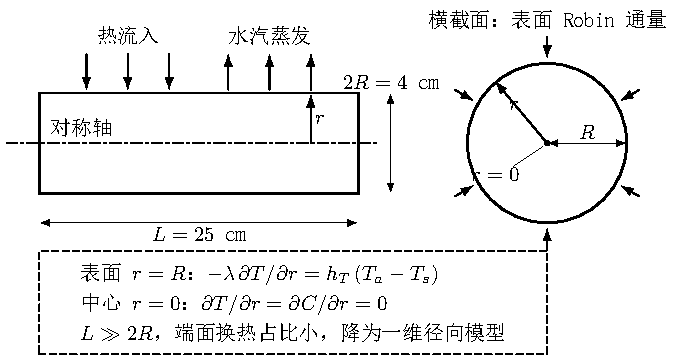
\includegraphics[width=0.9\textwidth,height=0.8\textheight,keepaspectratio]{../figures/tikz_cylinder_geometry.pdf}
  \caption{圆柱几何与边界条件}
  \label{fig:cylinder_geometry}
\end{figure}

降维后仅存两个通量方向，且二者相反：热量由热风经侧面传入、向轴心推进，
水分由内部向侧面迁移、再被气流带走（图~\ref{fig:cylinder_geometry}~标出这两个方向
与轴心、侧面两处边界）。
这一点在后文解释“表面先干、中心后干”与“表面先热、中心后热”
为何在时间尺度上差异悬殊时会多次用到。轴心处由对称性给出零通量条件，
它替代了通常意义上的第二个边界。

在半径 $r$ 处取厚度 $\mathrm{d}r$ 的环状控制体，对其写能量守恒：
单位时间内温度升高所需热量等于净流入的导热热量。以 $\rho(C)$、$c_p(C)$、$k(C)$
分别记密度、比热容与热传导系数，得

\begin{equation}
\rho(C)c_p(C)\frac{\partial T}{\partial t}
=\frac{1}{r}\frac{\partial}{\partial r}\!\left(r\,k(C)\frac{\partial T}{\partial r}\right),
\qquad 0<r<R(t).
\label{eq:heat_phys}
\end{equation}

水分一侧按假设（2）取 Fick 定律，以干基含水率 $C$ 为输运变量，
扩散系数 $D(C,T)$ 由附录经验式闭合：

\begin{equation}
\frac{\partial C}{\partial t}
=\frac{1}{r}\frac{\partial}{\partial r}\!\left(r\,D(C,T)\frac{\partial C}{\partial r}\right),
\qquad 0<r<R(t).
\label{eq:mass_phys}
\end{equation}

式~\eqref{eq:heat_phys}~与~\eqref{eq:mass_phys}~通过 $D$ 对 $T$ 的依赖
以及 $\rho,c_p,k$ 对 $C$ 的依赖双向耦合，只有在附录 2 的常物性闭合下
温度方程才退化为线性。

\subsection{边界条件与传递驱动力}

轴心处对称性给出

\begin{equation}
\left.\frac{\partial T}{\partial r}\right|_{r=0}=0,
\qquad
\left.\frac{\partial C}{\partial r}\right|_{r=0}=0.
\label{eq:axis_bc}
\end{equation}

表面处热、质均按对流规律传递。热 Biot 数 $hR_0/k=25\times0.02/0.36=1.3889$
落在内外热阻相当的区间：既不能把药材视为温度均匀的集中参数体
（那要求 $Bi\ll1$），也不能把表面温度直接钉在热风温度上（那要求 $Bi\gg1$），
必须采用第三类边界条件。初始含水率下扩散系数约 $4.94\times10^{-9}$ m$^2$/s，
对应质 Biot 数 $h_mR_0/D\approx3.24$，同样两侧阻力均不可忽略。于是

\begin{equation}
-k(C)\left.\frac{\partial T}{\partial r}\right|_{r=R}
=h\left[T(R,t)-T_{\mathrm{air}}(t)\right],
\qquad
-D(C,T)\left.\frac{\partial C}{\partial r}\right|_{r=R}
=h_m\left[C(R,t)-W_{\mathrm{air}}(t)\right].
\label{eq:surface_bc}
\end{equation}

这一对边界条件即固体与周围介质间热质交换的标准形式\upcite{luikov1966surface}。
式~\eqref{eq:surface_bc}~右端的传质驱动力直接取空气含湿量
$W_{\mathrm{air}}(t)$，而非通常做法中的平衡含水率 $C_{\mathrm{eq}}$。
理由是引入 $C_{\mathrm{eq}}$ 必须给出吸附等温线，而题面与附录均未提供，
自拟等温线等于向模型注入题面之外的自由参数。这一读法还有一个必要的后果：
$W_{\mathrm{air}}$ 的平台值约 $0.05$ kg/kg，低于烘干阈值 $0.15$ kg/kg，
因此阈值必定在有限时间内达到，问题三与问题四的解存在。
若表面驱动浓度高于阈值，无论烘多久都不可能达标，题设本身就会失去意义。

初始条件由题面直接给出，$T(r,0)=28$ °C、$C(r,0)=2.55$ kg/kg，两者沿半径均匀。

\subsection{烘房条件与边界驱动数据}

式~\eqref{eq:surface_bc}~中的 $T_{\mathrm{air}}(t)$ 与 $W_{\mathrm{air}}(t)$
由附件 1 给出，覆盖 $0$ 至 $14400$ s、间隔 $60$ s 共 $241$ 个点，
中间时刻按线性插值取用。

\begin{figure}[!htbp]
  \centering
  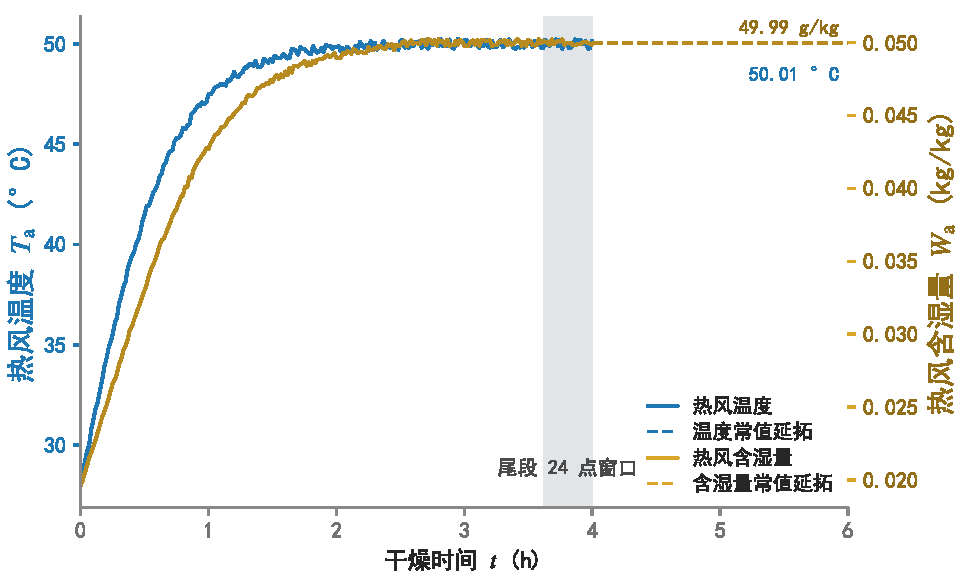
\includegraphics[width=0.9\textwidth,height=0.8\textheight,keepaspectratio]{../figures/fig_air_condition.pdf}
  \caption{热风温度与含湿量时程}
  \label{fig:air_condition}
\end{figure}

热风温度与含湿量两条曲线在约 $6000$ s 后都进入平台（图~\ref{fig:air_condition}）。
末 $24$ 个点的温度均值为 $50.0095$ °C、含湿量均值为 $0.049986$ kg/kg，
温度波动收在 $\pm0.26$ °C 以内；该段的线性拟合斜率仅 $0.06$ °C/h、
全段累计变化 $0.02$ °C，说明摆动是无趋势的随机散布而非残余升温。
问题三与问题四所需的时间跨度达五十余小时，远超附件 1 的覆盖范围，
故 $t>14400$ s 之后取上述均值作常数延拓。取均值而非末点，
是因为均值能抑制单点测量波动；取常数而非趋势外推，
是因为“恒温干燥”的字面含义就是此后烘房条件不再变化。

需要在结果之前就交代清楚的是这一延拓的权重：问题三 $57.4247$ h 的总时长中，
附件 1 实测覆盖的仅前 $4$ h，其余约 $93\%$ 的时间轴由延拓段支配。
第~\ref{sec:validation}~节的灵敏度分析给出该依赖的定量边界——
平台温度改变 $\pm0.5$ °C，烘干时长反向变化约 $1.6\%$，
折合约 $0.9$ h。因此本文给出的烘干时长应理解为“在恒温平台取该均值前提下”的
结果，而非无条件的绝对值。

两个附件提供的三条输入序列汇总于表~\ref{tab:input_stats}，
它们是本文全部边界条件与几何输入的唯一来源。

\begin{table}[H]
  \centering
  \caption{附件输入数据描述性统计}
  \label{tab:input_stats}
  \setlength{\tabcolsep}{4pt}
  \begin{tabular}{lrrrl}
  \toprule
  输入序列 & 样本数 & 起始或 $3$ h 值 & 末段代表值 & 末段值的取法 \\
  \midrule
  附件 1 热风温度 (°C)        & 241 & 50.1950 & 50.0095 & $13020$ s 后各点均值 \\
  附件 1 热风含湿量 (kg/kg)   & 241 & 0.04977 & 0.04999 & $13020$ s 后各点均值 \\
  附件 2 药材半径 (cm)        & 145 & 2.000   & 1.198   & 全程最小半径 \\
  \bottomrule
  \end{tabular}
\end{table}

表~\ref{tab:input_stats}~中附件 1 两行的“末段代表值”即上文用于常数延拓的平台均值，
$3$ h 处取值与之相差不足 $0.19$ °C 与 $0.0003$ kg/kg，
可见平台在附件 1 覆盖范围内已经建立，延拓并非把上升段的趋势外推出去。
附件 2 一行的取法不同：半径全程单调收缩，故第三列列出的是初值 $2.000$ cm、
末列为全程最小值 $1.198$ cm，中途 $6$ h 处为 $1.374$ cm，
其完整形态与对烘干时长的影响留到第~\ref{sec:p4}~节讨论。
三条序列的采样间隔分别为 $60$ s、$60$ s 与 $1800$ s，
中间时刻一律按线性插值取用，不做平滑或重采样。

\subsection{干质量拉格朗日坐标}

问题四中外半径 $R(t)$ 随时间收缩，物理域是移动边界问题。
若直接在 $r$ 上离散，网格须随时间重排，且方程中会出现网格运动带来的
伪对流项。规避这一困难的通行做法是把动边界映射到固定域上，
再以单个几何因子承载收缩\upcite{adrover2019shortcut}。本文改用干质量坐标

\begin{equation}
s=\left(\frac{r}{R(t)}\right)^{2}\in[0,1].
\label{eq:coord_def}
\end{equation}

选择平方而非线性比值，是因为 $s$ 正比于横截面积、从而正比于该半径以内包含的
干物质量。在假设（4）的仿射收缩下，每个物质点的 $r/R(t)$ 保持不变，
故每个 $s$ 值始终标记同一批干物质，坐标本身即拉格朗日坐标。

\begin{figure}[!htbp]
  \centering
  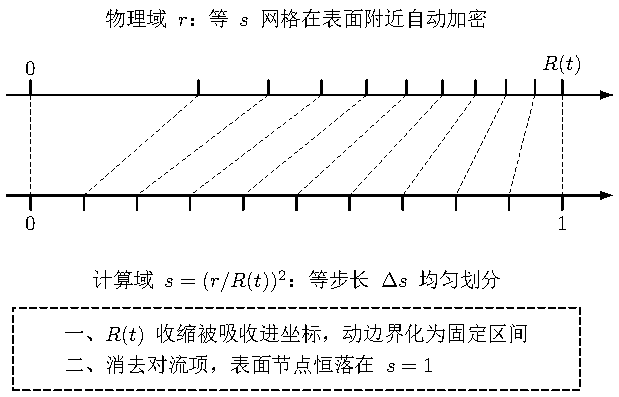
\includegraphics[width=0.9\textwidth,height=0.8\textheight,keepaspectratio]{../figures/tikz_coord_mapping.pdf}
  \caption{干质量坐标映射关系}
  \label{fig:coord_mapping}
\end{figure}

这一映射还带来两个附带好处（图~\ref{fig:coord_mapping}）。
其一，均匀的 $s$ 网格在物理空间自动向表面加密——表面正是浓度梯度最陡、
Robin 条件最需要分辨的位置；其二，$R(t)$ 收缩时全部节点随边界等比例内移，
网格拓扑不变。

设干骨架密度为 $\rho_s$。干物质总量守恒要求
$\rho_s(t)\pi R(t)^2L=\rho_{s0}\pi R_0^2L$，即

\begin{equation}
\rho_s(t)=\rho_{s0}\left(\frac{R_0}{R(t)}\right)^{2}.
\label{eq:rho_s}
\end{equation}

半径以内的干质量 $M_s(s)=\rho_s(t)\pi R(t)^2Ls=\rho_{s0}\pi R_0^2Ls$
与时间无关，这正是把 $s$ 用作输运坐标的依据。
由 $r=R\sqrt{s}$ 计算 $\partial/\partial r=(2\sqrt{s}/R)\partial/\partial s$
并代入式~\eqref{eq:mass_phys}，注意固定 $s$ 求时间导数时收缩项已被坐标吸收，
得到

\begin{equation}
\left.\frac{\partial C}{\partial t}\right|_{s}
=\frac{4}{R(t)^{2}}\frac{\partial}{\partial s}
\left(s\,D(C,T)\frac{\partial C}{\partial s}\right).
\label{eq:mass_s}
\end{equation}

温度方程作同样变换：

\begin{equation}
\rho(C)c_p(C)\left.\frac{\partial T}{\partial t}\right|_{s}
=\frac{4}{R(t)^{2}}\frac{\partial}{\partial s}
\left(s\,k(C)\frac{\partial T}{\partial s}\right).
\label{eq:heat_s}
\end{equation}

式~\eqref{eq:mass_s}~与~\eqref{eq:heat_s}~有三个值得指出的性质。
收缩在方程内部只留下系数 $4/R(t)^2$ 一处，不产生任何伪对流项
（$R(t)$ 另出现在下文式~\eqref{eq:bc_s}~的表面通量系数中，
两处都是随时间已知的标量因子，不引入新的微分项）；
柱坐标在 $r=0$ 处的 $1/r$ 奇点被 $s$ 因子吸收，轴心不再需要特殊处理；
求解域恒为 $[0,1]$，问题一至问题三取 $R\equiv R_0$ 即为定域情形，
四问因此可以共用同一份求解器。

边界条件随之改写。$s=0$ 处 $s\,\partial C/\partial s\to0$ 自动满足对称性，
$s=1$ 处由 $\partial/\partial r=(2/R)\partial/\partial s$ 得

\begin{equation}
-\frac{2k}{R}\left.\frac{\partial T}{\partial s}\right|_{s=1}
=h\left(T_R-T_{\mathrm{air}}\right),
\qquad
-\frac{2D}{R}\left.\frac{\partial C}{\partial s}\right|_{s=1}
=h_m\left(C_R-W_{\mathrm{air}}\right).
\label{eq:bc_s}
\end{equation}

对式~\eqref{eq:mass_s}~在 $[0,1]$ 上积分并代入式~\eqref{eq:bc_s}，
得到干质量加权平均含水率 $\bar C=\int_0^1C\,\mathrm{d}s$ 的全局平衡关系

\begin{equation}
\frac{\mathrm{d}\bar C}{\mathrm{d}t}
=-\frac{2h_m}{R(t)}\left(C_R-W_{\mathrm{air}}\right).
\label{eq:global_balance}
\end{equation}

式~\eqref{eq:global_balance}~不参与求解，但提供了一个与离散格式无关的
守恒检验：数值解的 $\bar C$ 变化率必须与表面通量逐步吻合。
第~\ref{sec:validation}~节用它给出的残差量级为 $10^{-10}$。

\subsection{节点中心有限体积离散}

在均匀 $s$ 网格上对散度形式方程作节点中心有限体积离散，内部节点由相邻界面通量差更新；轴心自然为零通量，表面半控制体直接装配 Robin 通量。后向 Euler 配合三次 Picard 迭代形成三对角方程组。该格式守恒且使表面值保持原始未知量；完整通量、端点半控制体推导见附录 B。
\iffalse

上述两个控制方程都是散度形式的非线性扩散方程，有限体积离散能逐个控制体地
满足守恒，正适合这类物性随解变化的问题\upcite{zhang2022fv}。
把 $[0,1]$ 划分为 $N$ 个等距区间，
节点 $s_i=i\Delta s$，$i=0,\dots,N$，
$\Delta s=1/N$。控制体以节点为中心：内部节点的控制体测度为 $\Delta s$，
两端节点为半格 $\Delta s/2$。

\begin{figure}[!htbp]
  \centering
  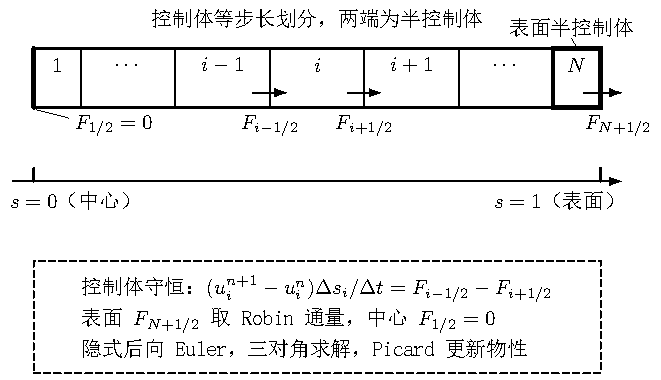
\includegraphics[width=0.9\textwidth,height=0.8\textheight,keepaspectratio]{../figures/tikz_fv_stencil.pdf}
  \caption{有限体积控制体与通量}
  \label{fig:fv_stencil}
\end{figure}

端点取半格是本格式的关键（图~\ref{fig:fv_stencil}）。表面值 $C_N$ 因此是
一个原始未知量而非插值得到的辅助量，Robin 条件直接写在 $s=1$ 上，
不需要虚拟节点或外推。若改用格心格式，表面落在控制体边界之外，
Robin 条件只能一阶近似，代价是可观的：$N=160$ 时格心格式的网格收敛残差
问题三停在 $1.046\times10^{-3}$、问题四停在 $7.424\times10^{-4}$，
均无法满足本文设定的 $5\times10^{-4}$ 相邻相对差判据；
换用节点中心格式后，同一网格上两问残差分别降到 $3.602\times10^{-4}$
与 $7.919\times10^{-5}$，无须靠加密网格硬压。

界面 $s_{i+1/2}=(i+1/2)\Delta s$ 处的扩散通量取相邻节点物性的算术平均

\begin{equation}
G_{i+1/2}=s_{i+1/2}\,D_{i+1/2}\,\frac{C_{i+1}-C_{i}}{\Delta s},
\qquad
D_{i+1/2}=\tfrac{1}{2}\left(D_i+D_{i+1}\right).
\label{eq:flux}
\end{equation}

对内部节点的控制体作平衡，得

\begin{equation}
\Delta s\,\frac{\mathrm{d}C_i}{\mathrm{d}t}
=\frac{4}{R^{2}}\left(G_{i+1/2}-G_{i-1/2}\right),
\qquad i=1,\dots,N-1.
\label{eq:fv_inner}
\end{equation}

轴心节点的控制体为 $[0,\Delta s/2]$，其内侧界面处 $s_{1/2}$ 因子使通量
自动为零量级，无须额外条件：

\begin{equation}
\frac{\Delta s}{2}\frac{\mathrm{d}C_0}{\mathrm{d}t}
=\frac{4}{R^{2}}G_{1/2}.
\label{eq:fv_axis}
\end{equation}

表面节点的控制体为 $[1-\Delta s/2,1]$，外侧界面即物理表面，
其通量由式~\eqref{eq:bc_s}~给出的 $-(h_mR/2)(C_N-W_{\mathrm{air}})$ 代入，
连同 $4/R^2$ 与 $s=1$ 整理后为

\begin{equation}
\frac{\Delta s}{2}\frac{\mathrm{d}C_N}{\mathrm{d}t}
=-\frac{4}{R^{2}}G_{N-1/2}-\frac{2h_m}{R}\left(C_N-W_{\mathrm{air}}\right).
\label{eq:fv_surface}
\end{equation}

式~\eqref{eq:fv_surface}~表明 Robin 系数以 $2h_m/R$ 的形式
直接进入系数矩阵的对角元，其与 $W_{\mathrm{air}}$ 的乘积
则进入右端项。因此边界条件是按其原始形式代入的，无需借助虚拟节点外推，
不引入额外的边界近似；控制体内部的通量 $G_{N-1/2}$ 仍带有与内节点同阶的
截断误差。温度方程的离散完全平行：把式~\eqref{eq:flux}~至
\eqref{eq:fv_surface}~中的 $D$ 换成 $k$、$h_m$ 换成 $h$、$W_{\mathrm{air}}$
换成 $T_{\mathrm{air}}$，并在时间导数项前保留因子 $\rho(C)c_p(C)$ 即可。

\fi
\subsection{时间推进与非线性处理}

物性依赖解本身，方程是非线性的。显式格式在 $\Delta s$ 加密时稳定性条件
过于苛刻，故采用后向 Euler 隐式格式\upcite{cruz2019implicit}——它对系数
冻结后的线性问题无条件稳定，非线性情形下的稳定性不由此自动保证，
需由下文的时间步无关性检验实测确认——并以 Picard 迭代处理非线性：
每个时间步内先用上一迭代的温度更新水分场，再用更新后的含水率求解温度场，
顺序迭代三次。三次的依据是第三次迭代引起的相对变化已不影响结果的第四位小数，
即不改变本文各表的制表精度；这是按制表位数选定的实用停止准则，
而非收敛到浮点精度极限的断言。

离散后系数矩阵为三对角，用带状直接解法求解，单步计算量与 $N$ 成正比。
生产算例取 $N=160$。这个数选取自两个约束的交集：网格无关性要求
相邻加密的 $t_{\mathrm{dry}}$ 相对差小于 $5\times10^{-4}$，
而制表要求 $r=0$、$0.5$、$1$、$1.5$、$2$ cm 五个位置恰好落在节点上。
后一条要求 $N$ 是 $16$ 的倍数：由式~\eqref{eq:coord_def}，
这五个半径对应 $s=0$、$0.0625$、$0.25$、$0.5625$、$1$，
分母最大为 $16$。$N=160$ 同时满足两者，制表值全部为节点原值、
不含任何空间插值误差。

时间步长按各问的制表分辨率取值：问题一的 $1800$ s 预热段取
$\Delta t=0.25$ s，问题二的 $3$ h 算例取 $0.5$ s，
问题三与问题四的数十小时全过程算例取 $1$ s。
第~\ref{sec:validation}~节的时间步无关性检验表明 $\Delta t$ 由 $4$ s
减到 $0.5$ s 时 $t_{\mathrm{dry}}$ 仅变化 $3\times10^{-3}$ h。

\subsection{烘干时长的判定}

问题三与问题四要求的不是给定时刻的场，而是满足烘干要求的首个时刻。
题面“各处的水分浓度应低于 $0.15$ kg/kg”作用在空间最大值上，故

\begin{equation}
t_{\mathrm{dry}}=\min\left\{t:\ \max_{0\le r\le R(t)}C(r,t)<C_{\mathrm{th}}\right\},
\qquad C_{\mathrm{th}}=0.15~\text{kg/kg}.
\label{eq:tdry_def}
\end{equation}

式~\eqref{eq:tdry_def}~写在物理坐标 $r$ 上，与题面的表述一致；
由于 $r=R(t)\sqrt{s}$ 在 $[0,R(t)]$ 与 $[0,1]$ 之间是双射，
对 $r$ 取最大值与对求解坐标 $s$ 取最大值给出同一个值，
程序在 $s$ 网格上扫描即可，本文两种写法可互换使用。
该最大值直接使用需在每个输出步扫描全域。
本文所有算例的含水率剖面均沿半径单调递减：初始场均匀，表面是唯一的水分出口，
故内部含水率不低于外部；第~\ref{sec:validation}~节实测的最大正向径向梯度为
$2.22\times10^{-15}$，与浮点舍入同量级，未出现方向相反的梯度。
在此单调性成立的前提下空间最大值取于中心，式~\eqref{eq:tdry_def}~可标量化为
$C(0,t)<C_{\mathrm{th}}$。这一标量化依据的是各算例的实测单调性，
而非对任意参数组合成立的证明；程序仍按全域最大值判定，
单调性只用于解释为何两者给出相同结果。设输出步 $t_j$ 与 $t_{j+1}$ 分别位于阈值两侧，
按线性插值定位

\begin{equation}
t_{\mathrm{dry}}=t_j+\left(t_{j+1}-t_j\right)
\frac{C(0,t_j)-C_{\mathrm{th}}}{C(0,t_j)-C(0,t_{j+1})}.
\label{eq:tdry_interp}
\end{equation}

必须强调判据施加在最大值而非截面平均值上。本文算得的干质量加权平均含水率
在 $36$ h 附近即已降到 $0.1499$ kg/kg，若误用均值判据将得到约 $36$ h 的答案，
比逐点判据短三成以上；而该时刻中心处仍有 $0.1858$ kg/kg，
药材内部远未达到烘干要求。这一区分在本题的量级下不是细节。

\section{问题一：基于常物性闭合的预热平衡阶段模型}
\label{sec:p1}

\subsection{物性闭合与输运尺度判别}

问题一取附录 2 的物性：密度 $\rho=820$ kg/m$^3$、比热容 $c_p=2600$ J/(kg·K)、
热传导系数 $k=0.36$ W/(m·K) 三者均为常数，只有水分扩散系数依赖含水率，

\begin{equation}
D(C)=7\times10^{-9}\,\mathrm{e}^{-0.89/C}\quad\text{m}^2/\text{s}.
\label{eq:D_app2}
\end{equation}

半径固定为 $R_0=0.02$ m。于是式~\eqref{eq:heat_s}~的系数全为常数、
温度方程成为线性方程，而式~\eqref{eq:mass_s}~仍因 $D(C)$ 而非线性。
这一非对称性是问题一独有的机会：温度场可以另求解析解，
从而构造一条不依赖本文离散格式的校验通道。

热扩散率

\begin{equation}
\alpha=\frac{k}{\rho c_p}=\frac{0.36}{820\times2600}
=1.6886\times10^{-7}\quad\text{m}^2/\text{s},
\label{eq:alpha}
\end{equation}

预热段终点的热 Fourier 数 $\mathrm{Fo}=\alpha t/R_0^2=0.759850$，量级为 $1$，
说明 $1800$ s 恰好是热扰动穿透半径所需的时间尺度。水分一侧，初始含水率下
$D(2.55)=4.937\times10^{-9}$ m$^2$/s，比 $\alpha$ 小 $34.2$ 倍，
质 Fourier 数仅 $0.0222$。扩散长度按 $\sqrt{Dt}$ 缩放，
两者相差 $\sqrt{34.2}\approx5.85$ 倍，即同样时间内湿分扰动只能推进热扰动
约六分之一的距离。再配合 $Bi=1.3889$ 与 $Bi_m=3.24$，可对本阶段的输运结构作出主要尺度判断：
热一侧 $Bi$ 为 $O(1)$，内外热阻相当，表面既非等温也非绝热；
质一侧 $Bi_m=3.24$ 明显大于 $1$ 且约为 $Bi$ 的 $2.3$ 倍，
表面对流不是控制环节，内部扩散阻力才是，这与湿分只在薄壳内变化的结果一致。
两侧的推进速度相差近六倍。这四个数各自只在其定义的机制上有效，
给出的是量级判断，不替代耦合方程的完整求解。

\subsection{完整模型}

问题一的完整模型为式~\eqref{eq:heat_s}~与~\eqref{eq:mass_s}~取 $R\equiv R_0$，

\begin{align}
\rho c_p\frac{\partial T}{\partial t}
&=\frac{4k}{R_0^{2}}\frac{\partial}{\partial s}
\left(s\frac{\partial T}{\partial s}\right),
\label{eq:p1_heat}\\
\frac{\partial C}{\partial t}
&=\frac{4}{R_0^{2}}\frac{\partial}{\partial s}
\left(s\,D(C)\frac{\partial C}{\partial s}\right),
\label{eq:p1_mass}
\end{align}

配以式~\eqref{eq:bc_s}~的表面 Robin 条件、式~\eqref{eq:D_app2}~的扩散系数闭合
与题给均匀初值 $T=28$ °C、$C=2.55$ kg/kg，时间区间 $[0,1800]$ s，
其中 $T_{\mathrm{air}}$、$W_{\mathrm{air}}$ 由附件 1 插值。
按第~\ref{sec:model}~节的格式取 $N=160$、$\Delta t=0.25$ s 推进求解。

\subsection{结果与制表}

\begin{figure}[!htbp]
  \centering
  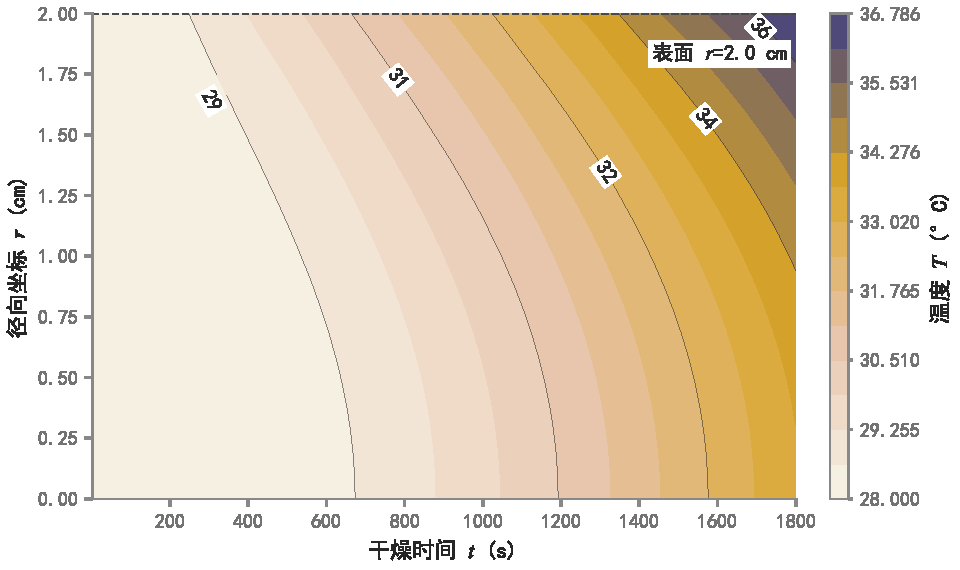
\includegraphics[width=0.9\textwidth,height=0.8\textheight,keepaspectratio]{../figures/fig_q1_field_T.pdf}
  \caption{问题一温度场分布}
  \label{fig:q1_field_T}
\end{figure}

图~\ref{fig:q1_field_T}~的等温线自表面向中心平移，前 $300$ s 内几乎贴着表面，
此后逐步深入。$1800$ s 时表面温度 $36.7857$ °C、中心 $33.5757$ °C，
内外温差 $3.2100$ °C，尚未抹平；同期热风为 $41.513$ °C，
表面仍比热风低 $4.7$ °C。三个数字共同说明预热段结束时药材既未达到热风温度、
内部也未均温，这正是 $\mathrm{Fo}\approx0.76$、$Bi\approx1.39$ 的应有形态。

\iffalse
\begin{figure}[!htbp]
  \centering
  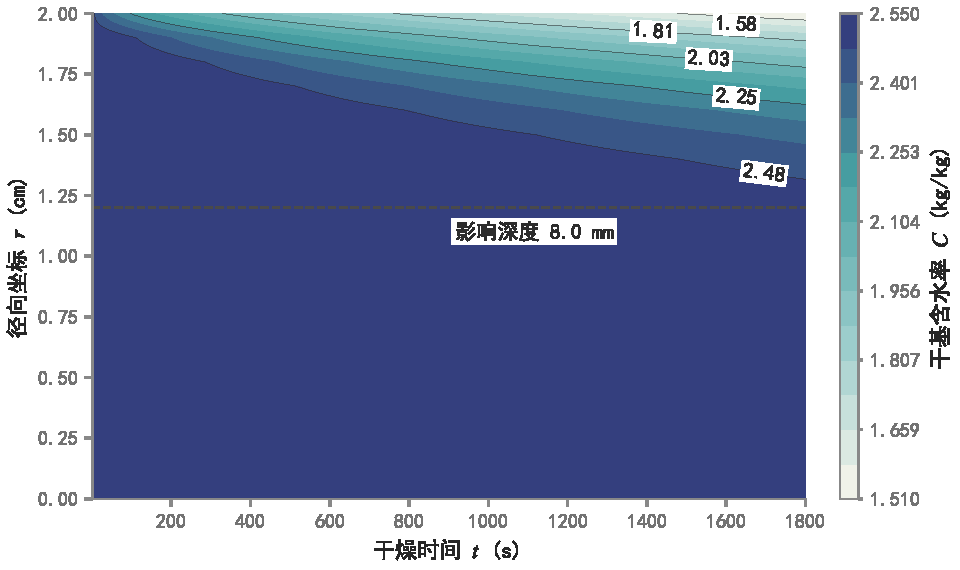
\includegraphics[width=0.9\textwidth,height=0.8\textheight,keepaspectratio]{../figures/fig_q1_field_C.pdf}
  \caption{问题一含水率场分布}
  \label{fig:q1_field_C}
\end{figure}

含水率场的形态与此形成对照。在图~\ref{fig:q1_field_C}~中等值线始终挤在
最外侧，中心大片区域保持初值。$1800$ s 时 $r\le1.0$ cm 处的降幅不足 $0.5\%$，
按干质量加权计最外 $4$ mm 承担了全部失水的 $84.4\%$，而表面已由 $2.5500$ 降到
$1.5103$ kg/kg。这是式~\eqref{eq:D_app2}~给出的扩散系数比热扩散率小
一个半数量级的直接结果，不是数值上的凝滞。

\begin{figure}[!htbp]
  \centering
  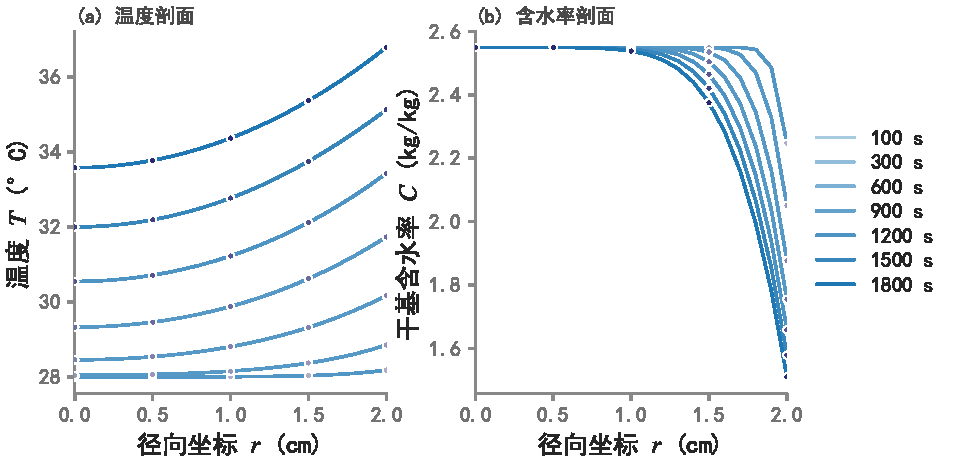
\includegraphics[width=0.9\textwidth,height=0.8\textheight,keepaspectratio]{../figures/fig_q1_profiles.pdf}
  \caption{问题一径向剖面族}
  \label{fig:q1_profiles}
\end{figure}

把两个场按七个制表时刻切成剖面族，可以看得更细
（图~\ref{fig:q1_profiles}，散点标出五个制表半径）。
温度剖面整体抬升、形状相似，属于典型的渗透型加热；
含水率剖面则是根部固定在 $2.55$、只有末端被向下拉的“折线”形态，
干燥前沿尚未离开表层。五个制表半径在 $N=160$ 的网格上对应
$s=0$、$0.0625$、$0.25$、$0.5625$、$1$，恰好落在节点 $i=0,10,40,90,160$ 上，
故下面两张表的数值是节点原值，不含空间插值误差。
\fi

\begin{table}[H]
  \centering
  \caption{问题一各时刻各位置温度（°C）}
  \label{tab:q1_T}
  \begin{tabular}{cccccc}
  \toprule
  时刻 (s) & $r=0$ cm & $r=0.5$ cm & $r=1.0$ cm & $r=1.5$ cm & $r=2.0$ cm \\
  \midrule
  100  & 28.0001 & 28.0004 & 28.0041 & 28.0328 & 28.1802 \\
  300  & 28.0410 & 28.0637 & 28.1516 & 28.3683 & 28.8491 \\
  600  & 28.4538 & 28.5364 & 28.8043 & 29.3162 & 30.1655 \\
  900  & 29.3248 & 29.4587 & 29.8759 & 30.6165 & 31.7306 \\
  1200 & 30.5432 & 30.7102 & 31.2228 & 32.1129 & 33.4279 \\
  1500 & 31.9962 & 32.1871 & 32.7664 & 33.7465 & 35.1204 \\
  1800 & 33.5757 & 33.7723 & 34.3644 & 35.3624 & 36.7857 \\
  \bottomrule
  \end{tabular}
\end{table}

表~\ref{tab:q1_T}~沿半径严格递增、沿时间严格递增，
$100$ s 时中心仅升温 $0.0001$ °C，说明热扰动此时还没有到达轴心。
这些温度有一个已知的偏向需要一并交代：按假设（3）本文未显式建模
汽化潜热引起的表面降温，实际表面温度应略低于表中数值。
第~\ref{sec:validation}~节的灵敏度结果界定了该简化的后果——
对流换热系数变化 $\pm20\%$ 时烘干时长仅改变约 $0.03\%$，
表面热阻并非控制环节，故表面温度的估计偏差不会传导为时长的显著偏差。

\begin{table}[H]
  \centering
  \caption{问题一各时刻各位置水分浓度（kg/kg）}
  \label{tab:q1_C}
  \begin{tabular}{cccccc}
  \toprule
  时刻 (s) & $r=0$ cm & $r=0.5$ cm & $r=1.0$ cm & $r=1.5$ cm & $r=2.0$ cm \\
  \midrule
  100  & 2.5500 & 2.5500 & 2.5500 & 2.5500 & 2.2473 \\
  300  & 2.5500 & 2.5500 & 2.5500 & 2.5492 & 2.0509 \\
  600  & 2.5500 & 2.5500 & 2.5500 & 2.5353 & 1.8770 \\
  900  & 2.5500 & 2.5500 & 2.5497 & 2.5045 & 1.7548 \\
  1200 & 2.5500 & 2.5500 & 2.5482 & 2.4646 & 1.6586 \\
  1500 & 2.5500 & 2.5499 & 2.5445 & 2.4206 & 1.5788 \\
  1800 & 2.5500 & 2.5497 & 2.5383 & 2.3755 & 1.5103 \\
  \bottomrule
  \end{tabular}
\end{table}

含水率一侧的分布则极不均匀。表~\ref{tab:q1_C}~的中心列七个时刻全部
保持 $2.5500$，$r=0.5$ cm 处直到 $1500$ s 才在第四位小数上出现变化，
而表面列已下降 $1.0397$ kg/kg。按式~\eqref{eq:global_balance}~所用的
干质量加权计，$1800$ s 时截面平均含水率为 $2.2936$ kg/kg，
即预热段总共排出初始水分的 $10.06\%$。
两张表并读可以给预热阶段定性：它主要是升温过程，
脱水虽已开始却局限在表层，中心区域尚未启动。
$1800$ s 内每隔 $1$ s、每隔 $0.1$ cm 的完整结果见 \verb|result1.xlsx|，
温度与水分浓度各一张工作表，每表 $1800$ 行 $\times$ $22$ 列。
后文交付文件的列数一律按含时间列的表头长度计，
$22$ 列即一列时间标签加 $0$ 至 $2.0$ cm 共 $21$ 个半径列。

\subsection{热、质推进的尺度分离}

热扰动已贯穿半径而湿分仍局限于表层，故预热的主要作用是升温；完整热湿推进图见附录 B。
\iffalse

\begin{figure}[!htbp]
  \centering
  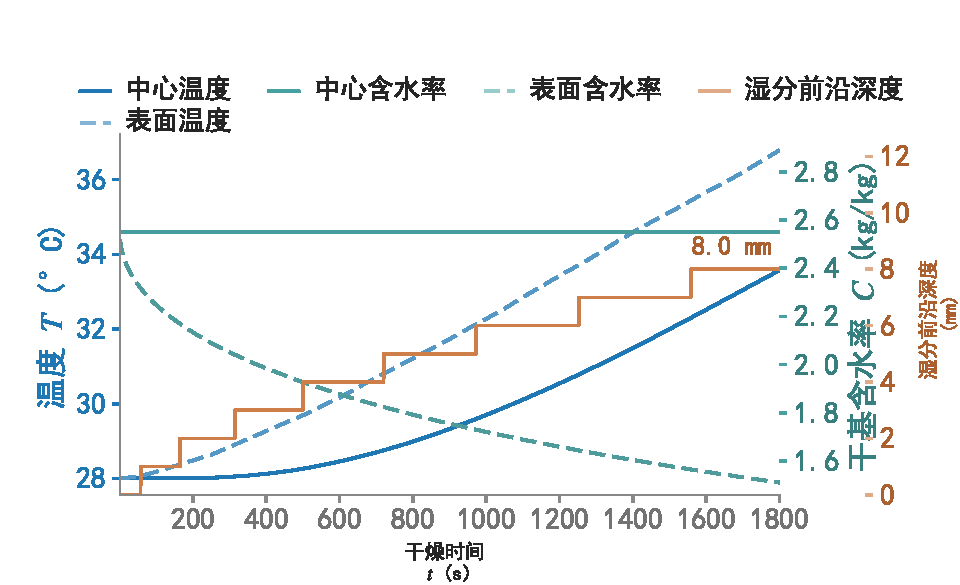
\includegraphics[width=0.9\textwidth,height=0.8\textheight,keepaspectratio]{../figures/fig_q1_penetration.pdf}
  \caption{问题一热湿推进对比}
  \label{fig:q1_penetration}
\end{figure}

热扰动在 $1800$ s 内已贯穿整个半径，而湿扰动只走完不到半个半径
（图~\ref{fig:q1_penetration}~把中心与表面的温度、含水率时程和湿分渗透深度
画在一起）。温度一侧，中心曲线在约 $200$ s 后开始明显抬升，
到 $1800$ s 已跟随表面上升、两条线的间距稳定在 $3$ °C 量级，
即热扰动已走完全程。含水率一侧，表面曲线迅速下落，
中心曲线在整个时窗内是一条水平线。以偏离初值 $1\%$ 为前沿判据，
渗透深度到 $1800$ s 才推进到 $8.0$ mm，约为半径的五分之二，
且其中最外 $4$ mm 就占了失水量的八成以上。

这一对照给预热平衡阶段一个明确的物理定位：题面称之为“预热”是准确的，
该阶段的实质是把冷料整体升温至接近热风温度，脱水只在表层发生。
后续三问中真正决定烘干时长的湿分输运，在这一阶段还没有进入内部。
反过来说，问题二至问题四之所以需要几十小时，也正是因为湿分必须走完
热量在半小时内就走完的那段路程。

\subsection{解析解校验}

\fi
\subsection{解析解校验摘要}
常物性温度方程可由 Bessel--Duhamel 展开独立求解。采用减法变量 $T-T_{\mathrm{air}}$ 后，解析解与有限体积数值解的最大偏差仅 $5.224\times10^{-4}$ °C，说明温度方程及 Robin 边界的实现一致；完整推导和残差图见附录 B。
\iffalse

数值结果的可信度需要一条不依赖本文离散格式的独立通道来支撑。
由于式~\eqref{eq:p1_heat}~在附录 2 闭合下是常系数线性方程、
且与水分方程解耦，可以用特征函数展开配合 Duhamel 叠加求出解析解。
圆柱在对流边界下的瞬态导热本身有成熟的解析处理\upcite{guellal2009cylinder}，
非齐次与混合边界情形则须借助级数重构\upcite{zare2018analytic}，
本文的做法属于后者。

齐次 Robin 特征值问题 $\frac{1}{r}(rX')'+\zeta^2X/R_0^2=0$、$-kX'(R_0)=hX(R_0)$
给出以零阶 Bessel 函数为形状的特征函数与超越特征方程

\begin{equation}
X_n(r)=J_0\!\left(\zeta_n\frac{r}{R_0}\right),
\qquad
\zeta_nJ_1(\zeta_n)=\mathrm{Bi}\,J_0(\zeta_n),
\qquad
\lambda_n=\frac{\alpha\zeta_n^{2}}{R_0^{2}}.
\label{eq:eigen}
\end{equation}

式~\eqref{eq:eigen}~的根须在 $J_1$ 的相邻零点区间内逐个用 Brent 法求解；
若对全部模态使用统一初值迭代，多个模态会收敛到同一根。
本文求得 $\zeta_{1\sim6}=1.41847$、$4.16647$、$7.20848$、$10.30827$、
$13.42716$、$16.55454$，与文献参照值最大偏差 $3.96\times10^{-6}$，
基频衰减率 $\lambda_1=8.4937\times10^{-4}$ 1/s。

关键之处在于不能直接对 $T$ 做叠加。展开系数

\begin{equation}
A_n=\frac{2J_1(\zeta_n)}{\zeta_n\left[J_0^{2}(\zeta_n)+J_1^{2}(\zeta_n)\right]}
\label{eq:An}
\end{equation}

满足 $\sum_nA_nJ_0(\zeta_nr/R_0)=1$，但常数 $1$ 并不满足齐次 Robin 条件，
该展开非一致收敛、$A_n$ 只以 $\zeta_n^{-1/2}$ 衰减。$T_{\mathrm{air}}$ 缓变时的
准稳态响应会把这条慢收敛尾巴永久留在解里：实测偏差卡在 $0.196$ °C，
且仅随模态数 $M$ 以 $1/M$ 下降，增加模态几乎无效。

改令 $\theta(r,t)=T(r,t)-T_{\mathrm{air}}(t)$。$\theta$ 满足齐次 Robin 条件，
方程带源项 $-\dot T_{\mathrm{air}}(t)$，展开为

\begin{equation}
\theta(r,t)=\sum_{n=1}^{M}b_n(t)J_0\!\left(\zeta_n\frac{r}{R_0}\right),
\qquad
\dot b_n=-\lambda_nb_n-A_n\dot T_{\mathrm{air}}(t).
\label{eq:duhamel}
\end{equation}

附件 1 在 $60$ s 间隔上分段线性，故每段内 $\dot T_{\mathrm{air}}$ 为常数，
式~\eqref{eq:duhamel}~可逐段精确积分：

\begin{equation}
b_n^{j+1}=b_n^{j}\mathrm{e}^{-\lambda_n\Delta}
-A_n\frac{T_{\mathrm{air}}^{j+1}-T_{\mathrm{air}}^{j}}{\Delta}
\cdot\frac{1-\mathrm{e}^{-\lambda_n\Delta}}{\lambda_n},
\qquad
T=T_{\mathrm{air}}(t)+\theta,
\label{eq:bn_exact}
\end{equation}

其中 $\Delta=60$ s。减法形式下常数部分由前导项 $T_{\mathrm{air}}(t)$ 承担，
残余级数只需展开满足齐次边界的 $\theta$，系数以 $n^{-5/2}$ 衰减。

\begin{figure}[!htbp]
  \centering
  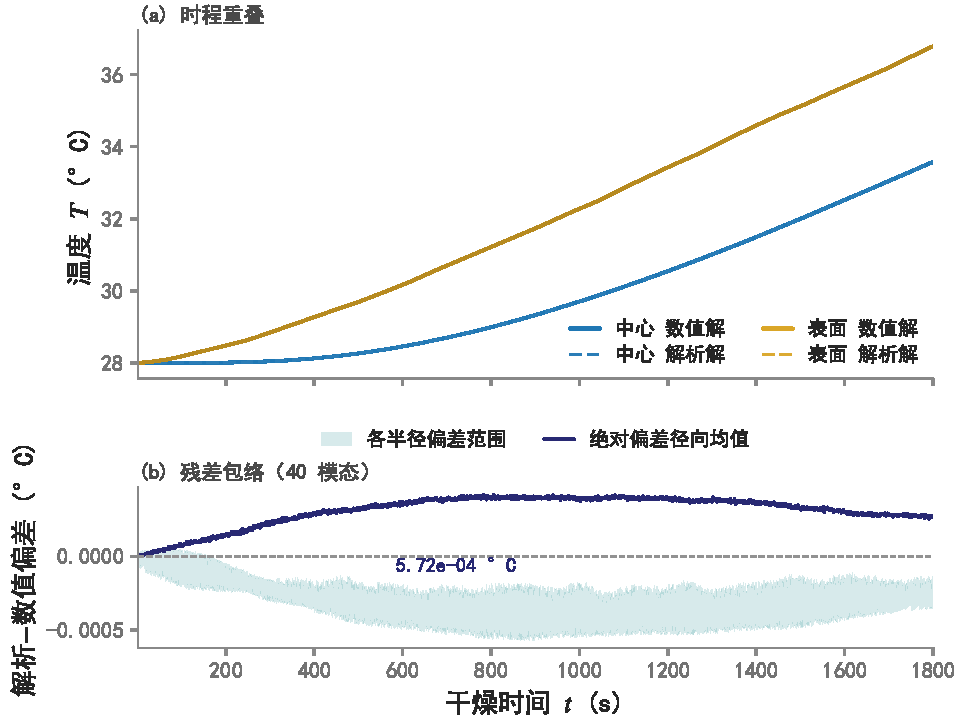
\includegraphics[width=0.9\textwidth,height=0.8\textheight,keepaspectratio]{../figures/fig_q1_analytic_val.pdf}
  \caption{解析解与数值解对比}
  \label{fig:q1_analytic_val}
\end{figure}

两条求解路径在全时窗、全半径上给出同一条温度曲线，最大偏差为
$5.224\times10^{-4}$ °C（图~\ref{fig:q1_analytic_val}~及其残差面板）。
该偏差取自 $M=40$ 个模态的截断；按 $M=6$、$12$、$20$、$40$ 逐档加模态，
偏差依次为 $1.838\times10^{-3}$、$5.565\times10^{-4}$、$5.257\times10^{-4}$、
$5.224\times10^{-4}$ °C，末两档只差 $3.3\times10^{-6}$ °C，
说明级数在 $M=40$ 处已收敛，残余偏差不来自截断。
它来自数值解自身的离散误差地板：把网格加密到 $N=640$、时间步减到 $0.05$ s 后，
同一模态数下偏差降到 $9.781\times10^{-5}$ °C，
即偏差随离散加密而下降、随模态数增加而不再变化，
两条求解路径在此精度内给出同一个解。
需要说明这一校验的范围：解析解与数值解共用同一组常物性和同一个 Robin 边界，
两者相符检验的是有限体积格式是否正确求解了该方程，属实现层面的独立校核，
不构成对模型物理设定（如不含潜热）的验证。
校验还有一处值得指出：附件 1 给出 $T_{\mathrm{air}}(0)=28.000000$ °C
与初始温度精确相等，故式~\eqref{eq:duhamel}~的初值 $b_n(0)\equiv0$，
本次比对检验的是完全由边界驱动的响应，不含初值瞬态带来的平凡吻合。
\fi

\section{问题二：基于变物性闭合的全过程耦合场模型}
\label{sec:p2}

\subsection{相对问题一的增量}

问题二把时间窗从预热段拉长到整个烘干过程，控制方程、坐标与离散格式
全部沿用第~\ref{sec:model}~节，唯一改变的是物性闭合：题面明示经验公式
统一采用附录 3，

\begin{align}
\rho(C)&=650+128C, &
c_p(C)&=1450+2736\,\frac{C}{C+1},
\label{eq:app3_rho_cp}\\
k(C)&=0.21+0.38\,\frac{C}{C+1}, &
D(C,T)&=2.4\times10^{-3}\,\mathrm{e}^{-0.45/C}\,\mathrm{e}^{-3850/T_K},
\label{eq:app3_k_D}
\end{align}

其中 $T_K=T+273.15$ 为热力学温度。式~\eqref{eq:app3_rho_cp}~与~\eqref{eq:app3_k_D}~
在代入时有三处必须辨明的读法。

其一，“统一采用”排除了按阶段切换物性的做法：即使在 $t\le1800$ s 的预热段
也应使用附录 3 而非附录 2。这直接导致问题二在 $1800$ s 处的数值与问题一不同，
后文专门给出对照与解释。

其二，$c_p$ 与 $k$ 中的组合 $C/(C+1)$ 是湿基含水率，不可简化为干基含水率 $C$。
初始状态下该组合等于 $0.7183$，而 $C=2.55$；若误用后者，
热传导系数将由 $0.48296$ 被放大到 $1.179$ W/(m·K)，超过实际值两倍以上。

其三，$D$ 中的 $\mathrm{e}^{-3850/T_K}$ 属于 Arrhenius 型，指数上的 $3850$
已含有活化能与气体常数之比（这与热风干燥中有效扩散系数随温度
呈指数增长的实测规律一致\upcite{singh2018potato}），因此温度必须用热力学温标。
若误用摄氏温标，在 $T=28$ °C 处 $\mathrm{e}^{-3850/28}$ 与
$\mathrm{e}^{-3850/301.15}$ 相差数十个数量级，扩散系数将完全失去意义。
此外 $\mathrm{e}^{-0.45/C}$ 在 $C\to0$ 时需以 $\max(C,10^{-12})$ 保护，
避免烘干末期的除零。

附录 3 只重新给出上述四项，没有重新给出对流换热系数与对流传质系数，
故按假设（5）这两个表面系数沿用附录 2 的 $h=25$ W/(m$^2$·K)、
$h_m=8\times10^{-7}$ m/s。这是不引入任何自由参数的唯一读法。

\subsection{变物性的实际变化幅度}

在 $50$ °C 下 $D$ 随 $C$ 从 $2.55$ 降至 $0.15$ 时由 $1.3471\times10^{-8}$ 降至 $8.0012\times10^{-10}$ m$^2$/s（约 $16.8$ 倍）；而 $28\to50$ °C 使初始 $D$ 提高 $2.39$ 倍。热物性的变化较温和，故变物性的主导影响来自扩散系数；完整轨迹见附录 B。
\iffalse

“变物性”三个字需要量化，否则无法判断它是否真的改变了问题的性质。

\begin{figure}[!htbp]
  \centering
  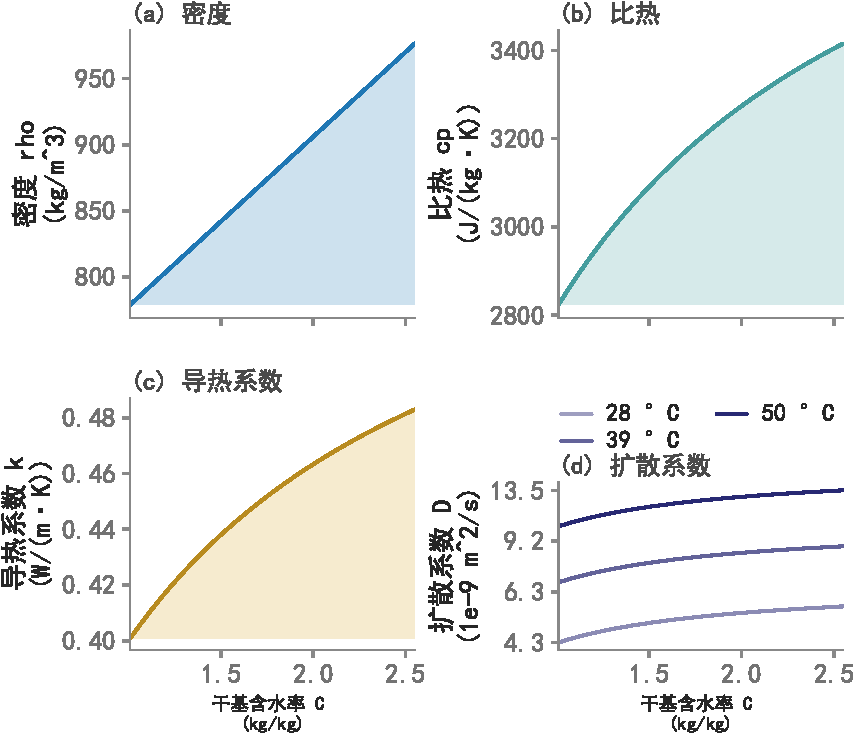
\includegraphics[width=0.8\textwidth,height=0.8\textheight,keepaspectratio]{../figures/fig_q2_props_evolution.pdf}
  \caption{附录三物性随含水率变化}
  \label{fig:q2_props_evolution}
\end{figure}

四项物性沿实际求解轨迹的变化幅度差别悬殊：三项热物性都是温和的单调下降，
只有扩散系数跨越一个数量级（图~\ref{fig:q2_props_evolution}）。
含水率由 $2.55$ 降到阈值 $0.15$ 的过程中，密度由 $976.4$ 降到 $669.2$ kg/m$^3$、
比热容由 $3415.3$ 降到 $1806.9$ J/(kg·K)、热传导系数由 $0.48296$ 降到
$0.25957$ W/(m·K)，三者都是不足一倍的温和变化，且方向一致地下降，
其对热扩散率 $\alpha=k/(\rho c_p)$ 的净影响被大幅抵消——
$\alpha$ 仅由 $1.4483\times10^{-7}$ 升到 $2.1467\times10^{-7}$ m$^2$/s。

扩散系数则完全不同。在 $50$ °C 的平台温度下，$D$ 由 $C=2.55$ 时的
$1.3471\times10^{-8}$ m$^2$/s 降到 $C=0.15$ 时的 $8.0012\times10^{-10}$ m$^2$/s，
降幅 $16.8$ 倍。这一强非线性是全局性的：干燥越接近完成，
水分越难迁移，烘干时长因此不与失水量成正比，而是在末段显著拖长。
本题所谓“变物性”的实质就集中在这一项上。

值得一并指出的是温度对 $D$ 的放大作用。同一含水率 $C=2.55$ 下，
$D$ 由 $28$ °C 时的 $5.6417\times10^{-9}$ 升到 $50$ °C 时的
$1.3471\times10^{-8}$ m$^2$/s，升高 $2.39$ 倍。
这说明热、质两个方程的耦合并非形式上的：预热把药材加热到平台温度，
其真正意义是把扩散系数提高一倍多，为后续脱水创造条件。

\fi
\subsection{烘房条件的时间覆盖}

问题二的时间窗超出附件 1 的覆盖范围，故按第~\ref{sec:model}~节的约定，
$t>14400$ s 后取末 $24$ 点平台均值 $T_{\mathrm{air}}=50.0095$ °C、
$W_{\mathrm{air}}=0.049986$ kg/kg 作常数延拓，绝不线性外推。
制表窗口 $3$ h 恰好落在附件 1 覆盖之内，因此表~\ref{tab:q2_T}~与
表~\ref{tab:q2_C}~的数值完全由实测边界驱动，不含延拓段的影响；
延拓的效力要到问题三与问题四才显现。

\subsection{结果与制表}

\begin{figure}[!htbp]
  \centering
  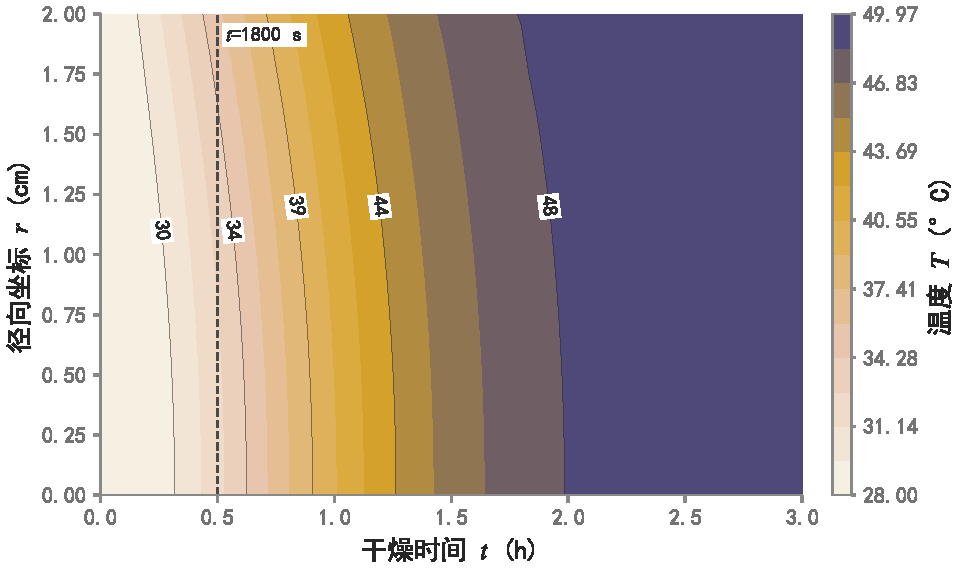
\includegraphics[width=0.74\textwidth,height=0.33\textheight,keepaspectratio]{../figures/fig_q2_field_T.pdf}
  \caption{问题二温度场分布}
  \label{fig:q2_field_T}
\end{figure}

图~\ref{fig:q2_field_T}~中等温线在前 $1$ h 仍明显倾斜，$2$ h 之后几乎垂直，
表明径向温差已被抹平、整根药材随热风同步变化。到 $3$ h 时内外温差
只有 $0.1169$ °C，中心与平台温度的差距为 $0.1600$ °C，
温度场实际上已进入准稳态。

\begin{figure}[!htbp]
  \centering
  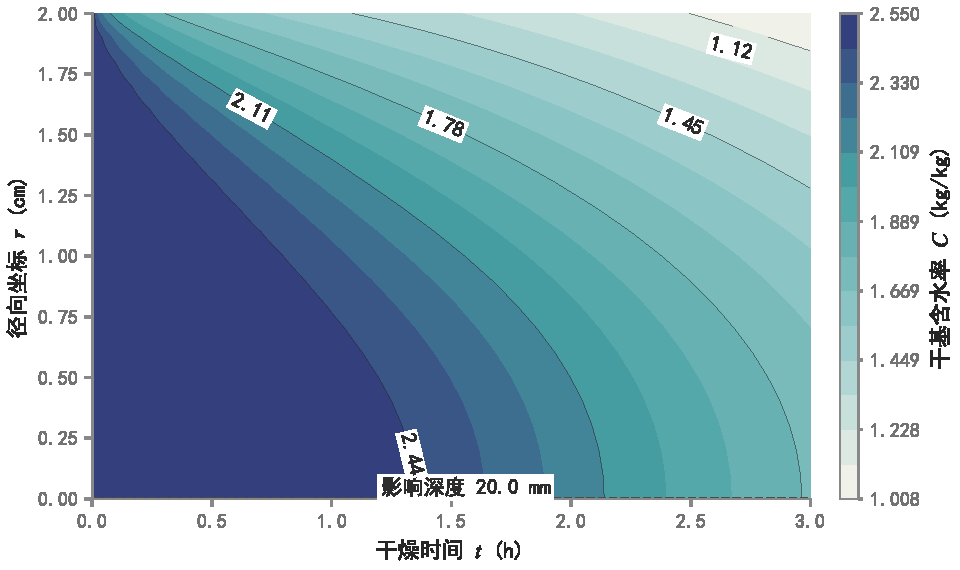
\includegraphics[width=0.74\textwidth,height=0.33\textheight,keepaspectratio]{../figures/fig_q2_field_C.pdf}
  \caption{问题二含水率场分布}
  \label{fig:q2_field_C}
\end{figure}

同一时窗内的含水率场呈现完全不同的形态。图~\ref{fig:q2_field_C}~显示
湿分梯度已从问题一的表皮薄层扩展到整个径向，等值线仍在向中心推进，
没有任何趋于均匀的迹象。到 $3$ h 时中心含水率只完成全程降幅的 $32.7\%$。
两张场图并读给出本题最重要的结构性判断：在这 $3$ h 窗口内热已基本平衡、
质仍在进行。这一判断能外推到后两问的数十小时全程，依据不止于本窗口：
第~\ref{sec:p3}~节的全程解表明温度场此后一直保持准稳态，
而第~\ref{sec:validation}~节的灵敏度排序中热风温度的影响
（$\pm0.5$ °C 对应 $\pm1.6\%$）远小于半径与传质系数。
因此后两问的烘干时长主要由传质控制，温度的作用是通过 Arrhenius 因子
设定扩散系数的水平。需要补充的是，传质本身并非纯内部扩散控制：
$h_m$ 减小 $20\%$ 使时长延长 $2.973\%$，表面对流阻力仍有可测量的份额。

\iffalse
\begin{figure}[!htbp]
  \centering
  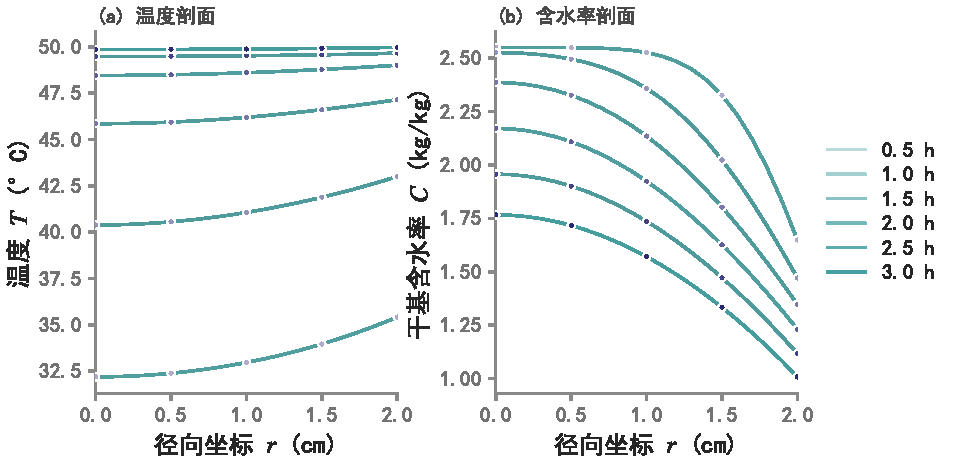
\includegraphics[width=0.9\textwidth,height=0.8\textheight,keepaspectratio]{../figures/fig_q2_profiles.pdf}
  \caption{问题二径向剖面族}
  \label{fig:q2_profiles}
\end{figure}

图~\ref{fig:q2_profiles}~的六条温度剖面逐条压平、间距递减，
与准稳态的判断一致；含水率剖面则保持“中心高、表面低”的单调形状整体下移，
斜率并未变缓。这一单调性是后文把逐点判据化为中心判据的依据。
\fi

\begin{table}[H]
  \centering
  \caption{问题二各时刻各位置温度（°C）}
  \label{tab:q2_T}
  \begin{tabular}{cccccc}
  \toprule
  时刻 (h) & $r=0$ cm & $r=0.5$ cm & $r=1.0$ cm & $r=1.5$ cm & $r=2.0$ cm \\
  \midrule
  0.5 & 32.1900 & 32.3828 & 32.9666 & 33.9614 & 35.4135 \\
  1.0 & 40.3816 & 40.5536 & 41.0605 & 41.8783 & 42.9977 \\
  1.5 & 45.8464 & 45.9345 & 46.1927 & 46.6048 & 47.1398 \\
  2.0 & 48.4500 & 48.4878 & 48.5982 & 48.7733 & 49.0032 \\
  2.5 & 49.4668 & 49.4790 & 49.5135 & 49.5653 & 49.6610 \\
  3.0 & 49.8495 & 49.8553 & 49.8746 & 49.9101 & 49.9664 \\
  \bottomrule
  \end{tabular}
\end{table}

表~\ref{tab:q2_T}~的内外温差由 $0.5$ h 的 $3.2235$ °C 收缩到 $3$ h 的
$0.1169$ °C，一个数量级半的衰减发生在两个半小时内。
与表~\ref{tab:q1_T}~同样需要说明的是：这些温度未计入汽化潜热引起的
表面降温，实际表面温度应略低于表值，第~\ref{sec:validation}~节给出的
$h$ 敏感度约 $0.03\%$ 表明该偏差不会传导为时长的显著变化。

\begin{table}[H]
  \centering
  \caption{问题二各时刻各位置水分浓度（kg/kg）}
  \label{tab:q2_C}
  \begin{tabular}{cccccc}
  \toprule
  时刻 (h) & $r=0$ cm & $r=0.5$ cm & $r=1.0$ cm & $r=1.5$ cm & $r=2.0$ cm \\
  \midrule
  0.5 & 2.5499 & 2.5489 & 2.5255 & 2.3257 & 1.6487 \\
  1.0 & 2.5256 & 2.4948 & 2.3578 & 2.0230 & 1.4711 \\
  1.5 & 2.3860 & 2.3256 & 2.1344 & 1.8020 & 1.3476 \\
  2.0 & 2.1708 & 2.1084 & 1.9236 & 1.6259 & 1.2311 \\
  2.5 & 1.9567 & 1.9006 & 1.7360 & 1.4720 & 1.1167 \\
  3.0 & 1.7662 & 1.7165 & 1.5702 & 1.3333 & 1.0081 \\
  \bottomrule
  \end{tabular}
\end{table}

中心含水率在 $0.5$ h 时几乎未动、$1$ h 后开始明显下降，
到 $3$ h 已降到 $1.7662$ kg/kg（表~\ref{tab:q2_C}）。这个“启动延迟”就是问题一观察到的
湿分渗透过程，只是在更长的时间窗里得以看到它抵达中心之后的行为。
$3$ h 内每隔 $1$ s、每隔 $0.1$ cm 的完整结果见 \verb|result2.xlsx|，
温度与水分浓度各一张工作表，每表 $10800$ 行 $\times$ $22$ 列。

\subsection{与问题一在同一时刻的差异}

问题二在预热段也采用附录 3，故 $1800$ s 的场值与问题一不同；这是物性闭合改变所致而非计算矛盾。完整常/变物性对照见附录 B。
\iffalse

因为问题二在预热段也使用附录 3，两问在 $1800$ s 处必然给出不同数值。
这不是计算不自洽，需要正面交代。

\begin{figure}[!htbp]
  \centering
  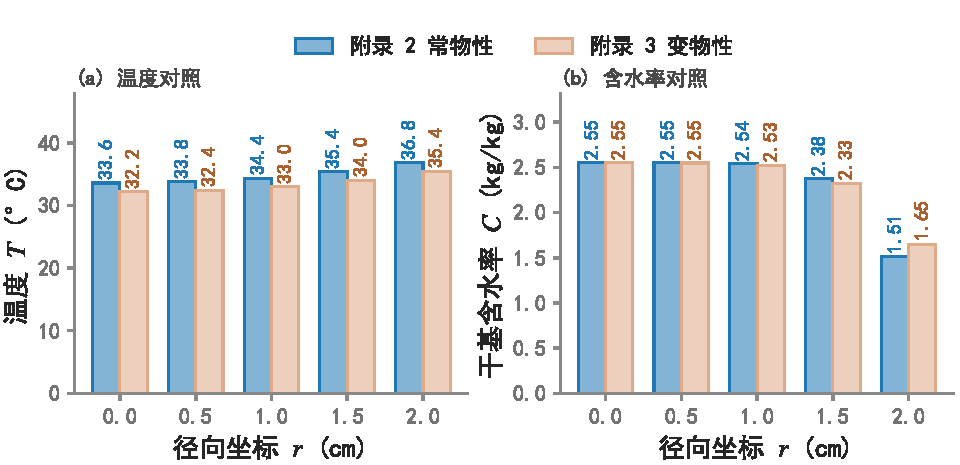
\includegraphics[width=0.9\textwidth,height=0.8\textheight,keepaspectratio]{../figures/fig_q1q2_contrast.pdf}
  \caption{常物性与变物性结果对照}
  \label{fig:q1q2_contrast}
\end{figure}

在 $1800$ s（即本节各表的 $0.5$ h 行）这一共同时刻上并排比较，
两问的温度差与含水率差方向相反
（图~\ref{fig:q1q2_contrast}~给出五个制表半径上的对照）。
温度一侧，问题二整体低于问题一，中心处
$32.1900$ °C 对 $33.5757$ °C，相差 $1.39$ °C。原因可以定量归因：
附录 3 在初始含水率下给出的 $\rho c_p$ 为 $3.335\times10^{6}$ J/(m$^3$·K)，
比附录 2 的 $2.132\times10^{6}$ 大 $56\%$，即同样热流下升温更慢；
热传导系数虽然也更大，但不足以抵消热容的增长，
净结果是热扩散率由 $1.6886\times10^{-7}$ 降到 $1.4483\times10^{-7}$ m$^2$/s。

含水率一侧的差异方向相反且更有意思：问题二的表面含水率 $1.6487$ 反而
高于问题一的 $1.5103$，而内部各点全部低于问题一（$1.0$ cm 处
$2.5255$ 对 $2.5383$）。这是因为附录 3 给出的扩散系数
$5.6417\times10^{-9}$ 比附录 2 的 $4.9377\times10^{-9}$ m$^2$/s 大 $14\%$，
内部水分向表面补充得更快，表面得以维持较高含水率，
而失水被摊到更深的范围。两问的截面平均含水率因此相差不大，
分别为 $2.2936$ 与 $2.2826$ kg/kg。以初始含水率 $C_0=2.55$ kg/kg 为分母折算
累计失水比例 $(C_0-\bar C)/C_0$，两问分别为 $10.06\%$ 与 $10.49\%$，
即问题二多排出 $0.43$ 个百分点。

这组对照说明附录 2 与附录 3 的差别不是简单的“更精确”或“数值更大”，
而是重新分配了热与质的相对快慢。后两问必须在附录 3 及附录 4 各自的
物性闭合下独立计算，不能从问题一的结果外推。
\fi

\section{问题三：基于阈值首达判据的烘干时长模型}
\label{sec:p3}

\subsection{相对问题二的增量}

问题三与问题二求解的是同一个初边值问题：附录 3 物性全程统一、
半径固定为 $R_0$、烘房条件按第~\ref{sec:model}~节的约定延拓。
唯一新增的内容是终止判据，即由“给定时刻求场”变为“给定场的条件求时刻”，
数学上是一个阈值首达型反问题，由式~\eqref{eq:tdry_def}~定义。
把该判据写成显式的优化形式，本问的目标函数与约束为

\begin{equation}
\begin{aligned}
&\min_{t>0}\ \ J_3(t)=t,\\
&\mathrm{s.t.}\ \ g_3(t)\equiv\max_{0\le r\le R_0}C(r,t)-C_{\mathrm{th}}<0,
\qquad C_{\mathrm{th}}=0.15~\text{kg/kg},\qquad R(t)\equiv R_0 .
\end{aligned}
\label{eq:p3_obj}
\end{equation}

式~\eqref{eq:p3_obj}~中目标函数 $J_3(t)=t$ 即待求的烘干时长，
$g_3(t)$ 为逐点达标裕度，$C_{\mathrm{th}}$ 为题面给定的含水率阈值。
可行域不含任何自由决策变量：含水率场 $C(r,t)$ 与温度场 $T(r,t)$
由式~\eqref{eq:mass_s}~至~\eqref{eq:bc_s}~的初边值问题在附录 3 物性闭合
式~\eqref{eq:app3_rho_cp}~与~\eqref{eq:app3_k_D}~下唯一确定，
故式~\eqref{eq:p3_obj}~的最优值就是阈值首达时刻 $t_{\mathrm{dry}}$，
与式~\eqref{eq:tdry_def}~等价。这也说明本问不是参数寻优问题：
$J_3$ 的下降只能靠正演求解推进时间轴，不能靠调整任何待定系数取得。

判据作用在哪个量上必须辨清。题面“药材各处的水分浓度应低于 $0.15$ kg/kg”
中的“各处”是逐点条件，作用在空间最大值上，而不是作用在截面平均值上。
本题量级下两者差别巨大：本文算得的干质量加权平均含水率在 $36$ h 时
已降到 $0.1499$ kg/kg，若误用均值判据将得到约 $36$ h 的答案，
比逐点判据少 $37\%$；而该时刻中心处仍有 $0.1858$ kg/kg，
比阈值高出 $23.9\%$，药材内部远未达标。

判据能否在有限时间内满足也需要事先检验。式~\eqref{eq:surface_bc}~的传质
驱动浓度为空气含湿量，其平台值 $0.049986$ kg/kg 低于阈值 $0.15$ kg/kg，
故平衡状态本身即满足要求，含水率可以持续下降到阈值以下。
这一条只排除了永不达标的情形，不足以给出有限的达标时刻；
$t_{\mathrm{dry}}$ 的有限性由下文的数值解直接给出——本算例在 $57.4247$ h 处首次达标。
反过来说，若驱动浓度高于阈值，则含水率的渐近下界高于 $0.15$，
无论烘多久都不可能达标，这时判据无解。

\subsection{单调性与判据的标量化}

含水率沿半径单调递减，故空间最大值位于中心；程序仍扫描全域最大值，以保证严格执行题意。完整径向剖面见附录 C。
\iffalse

\begin{figure}[!htbp]
  \centering
  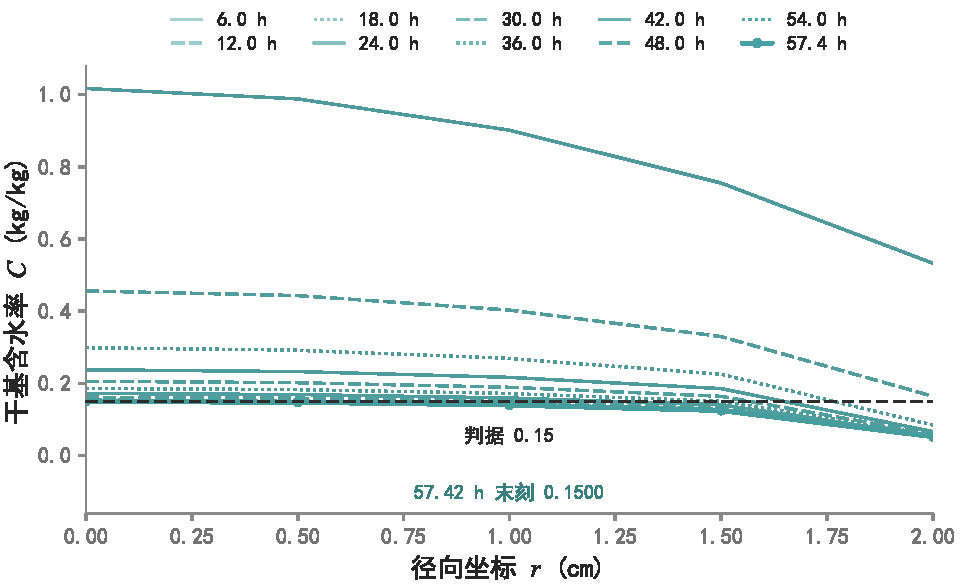
\includegraphics[width=0.9\textwidth,height=0.8\textheight,keepaspectratio]{../figures/fig_q3_profiles_6h.pdf}
  \caption{问题三每六小时径向剖面}
  \label{fig:q3_profiles_6h}
\end{figure}

每隔 $6$ h 取一条含水率剖面，可见所有剖面沿半径递减、形状逐条下移而不交叉
（图~\ref{fig:q3_profiles_6h}，图中标出 $0.15$ 阈值线）。数值上，
本算例全时空范围内的最大正向径向梯度为 $2.22\times10^{-15}$，
比单调性判据阈值 $10^{-9}$ 小六个量级，与双精度舍入同量级，
即未出现可分辨的正梯度。因此在本算例中空间最大值取于中心，
式~\eqref{eq:tdry_def}~的场判据与标量判据 $C(0,t)<0.15$ 给出相同的首达时刻，
可按式~\eqref{eq:tdry_interp}~在相邻 $60$ s 输出步之间线性插值定位。
这里的等价性来自实测单调性而非先验证明，故程序仍按全域最大值判定；
线性插值给出的是首达时刻的数值估计，其误差受输出步长 $60$ s 限制，
下文的时间步无关性检验给出该估计的稳定性。

图中还能读出另一件事：阈值线与各剖面的交点先出现在表面附近，
再逐条向中心移动，最后一条剖面在中心处刚好触到阈值。
这个几何图像正是“整根药材达标”与“中心达标”等价的直观来源。

\fi
\subsection{结果}

按 $N=160$、$\Delta t=1$ s 推进到第 $206\,760$ 步（即 $57.4333$ h）时判据首次满足，
在该步与前一输出步之间插值得

\begin{equation}
t_{\mathrm{dry}}=57.4247~\text{h}=2.3927~\text{d}.
\label{eq:tdry_q3}
\end{equation}

推进步数对应的时刻略迟于 $t_{\mathrm{dry}}$，二者相差不超过一个 $60$ s 输出步，
这是先跨过再回插的必然结果。
穿越确为首次：末输出步的 $\max_rC=0.149991$ 已低于阈值，
前一输出步为 $0.150008$ 仍高于阈值。全程离散守恒残差
$3.425\times10^{-10}$，说明式~\eqref{eq:global_balance}~的全局平衡
在数值解上逐步成立。

式~\eqref{eq:tdry_q3}~是一个条件式结论，其依赖关系在本节末尾定量给出：
$93.0\%$ 的时间轴由附件 1 末段平台的常数延拓提供边界条件，
该平台温度改变 $\pm0.5$ °C 时时长反向变化约 $1.6\%$。

\begin{figure}[!htbp]
  \centering
  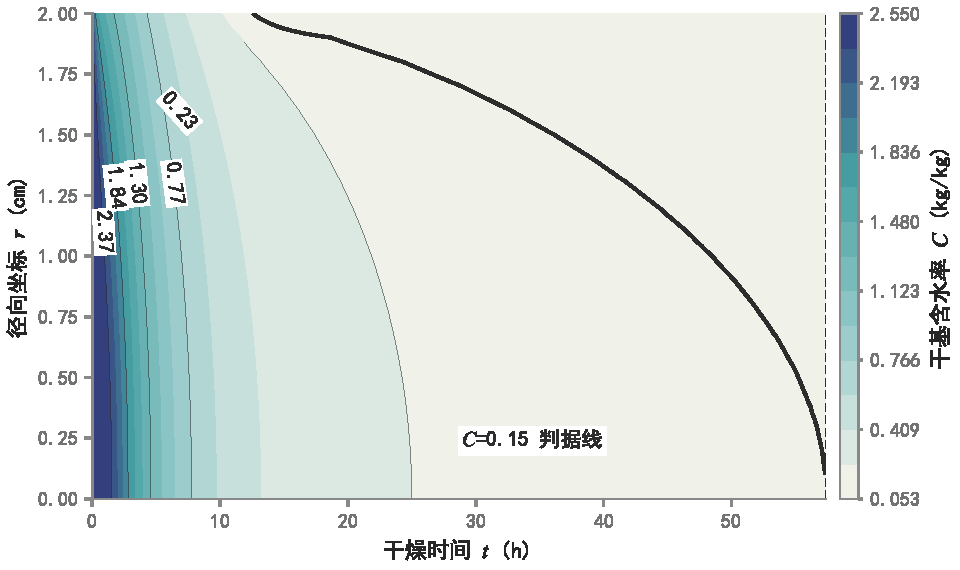
\includegraphics[width=0.9\textwidth,height=0.8\textheight,keepaspectratio]{../figures/fig_q3_field_C.pdf}
  \caption{问题三全程含水率场}
  \label{fig:q3_field_C}
\end{figure}

达标过程在时间上高度不均匀：$0.15$ 等值线在约 $12.6$ h 就抵达表面，
此后向中心推进的速度急剧变慢，最终在 $57.4247$ h 触及轴心——
这一时刻即式~\eqref{eq:tdry_q3}~的答案（图~\ref{fig:q3_field_C}~给出
$0$ 至 $57.42$ h 的全程含水率场并高亮该等值线）。等值线的减速形态与图~\ref{fig:q2_props_evolution}~中扩散系数
随含水率下降 $16.8$ 倍的强非线性直接对应：越接近达标，推进越慢。

式~\eqref{eq:tdry_q3}~落在题面给出的“一般持续 $2$ 至 $3$ 天”区间之内，
这是一条独立于本文模型的外部量级校核。

\begin{table}[H]
  \centering
  \caption{问题三烘干过程的水分浓度（kg/kg）}
  \label{tab:q3_C}
  \setlength{\tabcolsep}{4pt}
  \begin{tabular}{ccccccc}
  \toprule
  时间 (h) & $r=0$ cm & $r=0.5$ cm & $r=1.0$ cm & $r=1.5$ cm & $r=2.0$ cm & $\bar C$ \\
  \midrule
  6  & 1.0169 & 0.9881 & 0.9015 & 0.7550 & 0.5328 & 0.7817 \\
  12 & 0.4561 & 0.4431 & 0.4030 & 0.3297 & 0.1642 & 0.3367 \\
  18 & 0.2988 & 0.2915 & 0.2687 & 0.2253 & 0.0845 & 0.2270 \\
  24 & 0.2378 & 0.2327 & 0.2167 & 0.1855 & 0.0665 & 0.1858 \\
  30 & 0.2058 & 0.2018 & 0.1891 & 0.1640 & 0.0598 & 0.1639 \\
  36 & 0.1858 & 0.1825 & 0.1718 & 0.1503 & 0.0566 & 0.1499 \\
  42 & 0.1720 & 0.1691 & 0.1596 & 0.1406 & 0.0548 & 0.1401 \\
  48 & 0.1618 & 0.1591 & 0.1506 & 0.1334 & 0.0537 & 0.1328 \\
  54 & 0.1538 & 0.1514 & 0.1436 & 0.1276 & 0.0530 & 0.1270 \\
  烘干结束 57.4247 & 0.1500 & 0.1477 & 0.1402 & 0.1249 & 0.0526 & 0.1242 \\
  \bottomrule
  \end{tabular}
\end{table}

表~\ref{tab:q3_C}~的末行是烘干结束时刻，其余各处均已低于阈值，
中心值显示为 $0.1500$。这一显示值是四位小数舍入的结果，
未舍入值为 $0.149991$ kg/kg，已低于阈值；判据按未舍入值判定，
上一输出步的对应值为 $0.150008$ kg/kg，仍高于阈值，
两步之间正是插值定位的区间。表中同时给出干质量加权平均含水率一列，
便于读者核对前述均值判据与逐点判据的差别：第 $36$ h 行的 $\bar C=0.1499$
已达标而中心 $0.1858$ 未达标，两者的分歧一目了然。
同期温度在全部制表时刻、全部半径上均为 $50.0095$ °C，
四位小数下与平台温度不可分辨，故不单列温度表——
这再次印证问题二的判断：全程绝大部分时间里热已平衡，只有质在进行。
每隔 $60$ s、每隔 $0.1$ cm 的完整结果见 \verb|result3.xlsx|，
共 $3446$ 行 $\times$ $22$ 列，末行时刻已不早于 $t_{\mathrm{dry}}$。

\subsection{干燥动力学与烘房条件依赖}

\begin{figure}[!htbp]
  \centering
  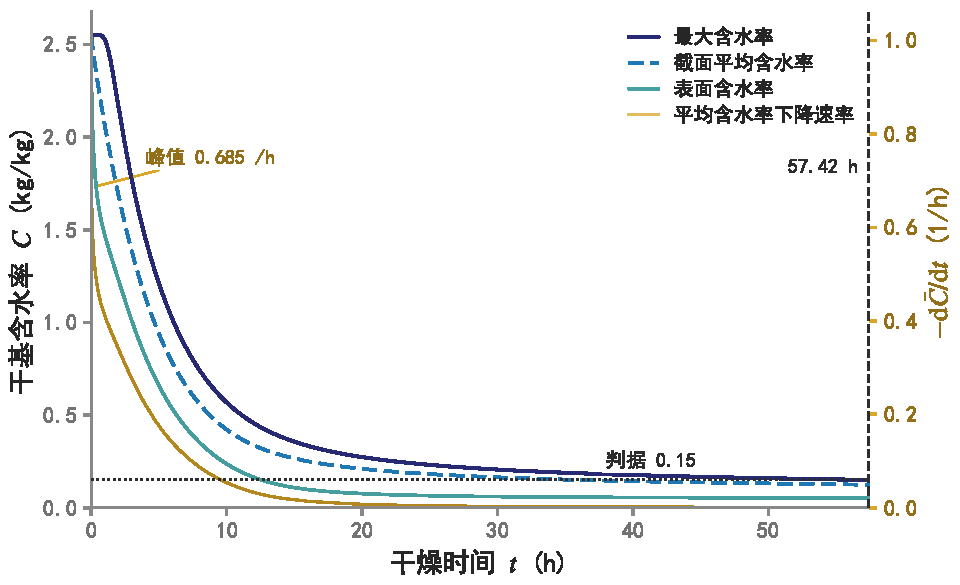
\includegraphics[width=0.9\textwidth,height=0.8\textheight,keepaspectratio]{../figures/fig_q3_drying_kinetics.pdf}
  \caption{问题三干燥动力学曲线}
  \label{fig:q3_drying_kinetics}
\end{figure}

本题工况下不存在恒速干燥段：三条含水率曲线全程不交叉，
干燥速率自始至终单调下降（图~\ref{fig:q3_drying_kinetics}~把中心、表面与
干质量加权平均含水率的时程与干燥速率画在双轴上）。这一“全程降速”特征与薄层热风干燥实验中
普遍观察到的形态一致\upcite{chigbo2024thinlayer,rodriguez2014thyme}，
说明本题工况下干燥速率始终由内部扩散控制，而非由表面汽化控制；表面含水率到 $18$ h 已降至 $0.0845$ kg/kg，
此后缓慢趋近空气含湿量 $0.05$ 的量级，成为内部水分的出口而不是限制环节。图中中心与平均两条曲线的间距
就是均值判据偏短的来源。

由于式~\eqref{eq:tdry_q3}~的时间跨度远超附件 1 的覆盖范围，
必须把该结果的条件性一并说清。附件 1 实测只覆盖前 $4$ h，
占总时长的 $7.0\%$；其余 $93.0\%$ 的时间轴由平台均值常数延拓段支配。
第~\ref{sec:validation}~节的单因子扰动给出该依赖的定量边界：
平台温度改变 $\pm0.5$ °C 时烘干时长反向变化约 $1.6\%$，折合约 $0.9$ h。
因此式~\eqref{eq:tdry_q3}~应理解为“在恒温平台取附件 1 末段均值前提下”
的烘干时长。作为鲁棒性对照，若改用末点值 $50.1650$ °C 而非均值
$50.0095$ °C 作延拓，两者相差 $0.1555$ °C，已被上述 $\pm0.5$ °C 的
扰动幅度覆盖。

\subsection{网格与时间步无关性}

$N=160$ 已满足相邻相对差 $5\times10^{-4}$ 判据；从 $\Delta t=4$ s 收至 $0.5$ s，$t_{\mathrm{dry}}$ 仅改变约 $3\times10^{-3}$ h。完整收敛图表见附录 C。
\iffalse

阈值首达时刻是一个由整条时程累积而来的量，比场值更容易受离散误差影响，
因此需要专门核查。

\begin{figure}[!htbp]
  \centering
  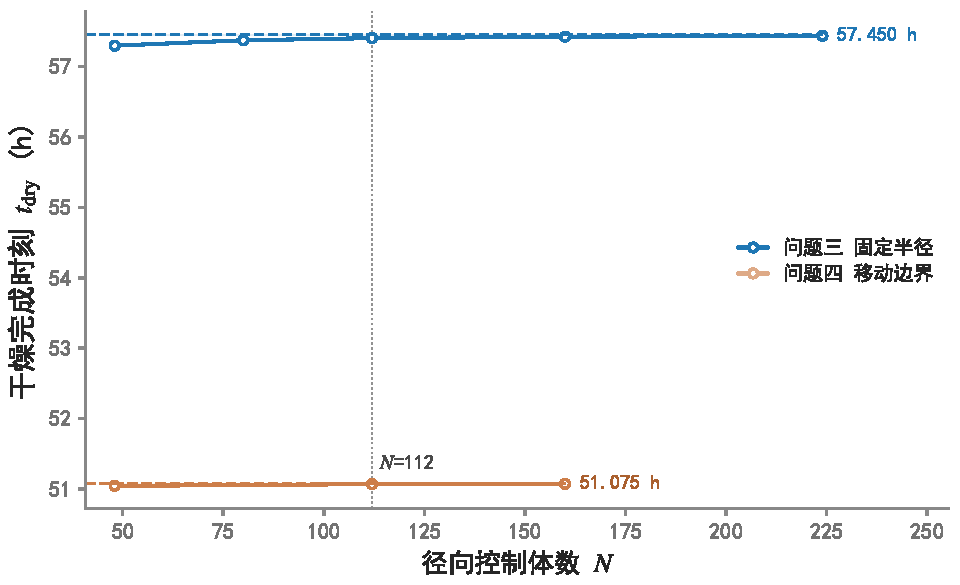
\includegraphics[width=0.9\textwidth,height=0.8\textheight,keepaspectratio]{../figures/fig_grid_convergence.pdf}
  \caption{网格收敛性检验}
  \label{fig:grid_convergence}
\end{figure}

两问的 $t_{\mathrm{dry}}$ 都随网格加密单调趋于稳定值，
相邻相对差在生产网格处已进入 $5\times10^{-4}$ 判据以内
（图~\ref{fig:grid_convergence}~给出两条收敛轨迹并标出该判据，
问题三一侧的具体数值列于表~\ref{tab:grid}）。

\begin{table}[H]
  \centering
  \caption{问题三网格收敛性}
  \label{tab:grid}
  \begin{tabular}{rrr}
  \toprule
  径向控制体数 $N$ & $t_{\mathrm{dry}}$ (h) & 相对前一档差 (\%) \\
  \midrule
  48  & 57.2968 & --     \\
  80  & 57.3738 & 0.1343 \\
  112 & 57.4040 & 0.0527 \\
  160 & 57.4247 & 0.0360 \\
  224 & 57.4370 & 0.0214 \\
  \bottomrule
  \end{tabular}
\end{table}

表~\ref{tab:grid}~的相对差列单调下降，末两档均已优于 $5\times10^{-4}$ 判据。
细化网格使 $t_{\mathrm{dry}}$ 单调略微变长，说明粗网格会低估烘干时长，
其机理是控制体过少时表面附近的陡梯度被抹平、表面通量被高估。
补充网格集 $N\in\{40,60,80,120,160\}$ 给出的相对差由 $1.390\times10^{-3}$
降到 $2.770\times10^{-4}$，同样单调，排除了收敛轨迹依赖于特定网格序列的可能。

\begin{table}[H]
  \centering
  \caption{问题三时间步收敛性}
  \label{tab:dt}
  \begin{tabular}{rr}
  \toprule
  时间步 $\Delta t$ (s) & $t_{\mathrm{dry}}$ (h) \\
  \midrule
  4.0 & 57.4067 \\
  2.0 & 57.4049 \\
  1.0 & 57.4040 \\
  0.5 & 57.4036 \\
  \bottomrule
  \end{tabular}
\end{table}

表~\ref{tab:dt}~在 $N=112$ 下固定空间网格单独考察时间步，
八倍的步长变化只改变 $3.0\times10^{-3}$ h，比表~\ref{tab:grid}~中同一档位
$N=112$ 的相邻网格差 $3.0\times10^{-2}$ h 小一个数量级。两表合起来说明
空间离散是误差主项、时间离散不是。生产配置 $N=160$、$\Delta t=1$ s 的
残余离散误差可由最密一档估计：$N=224$ 给出 $57.4370$ h，
与生产值相差 $0.0123$ h（约 $44$ s），相对量 $2.1\times10^{-4}$。
因此式~\eqref{eq:tdry_q3}~在小时量级上是稳定的，
但其末位小数不应按有效数字解读——本文保留四位小数只为便于复核，
可信区间由上述 $0.0123$ h 给出。
这也解释了后向 Euler 格式一阶时间精度在此并不构成限制：
烘干过程的时间尺度是数十小时，$1$ s 的步长相对之下极小。
\fi

\section{问题四：含收缩动边界的烘干时长模型}
\label{sec:p4}

\subsection{相对问题三的增量}

问题四相对问题三只增加两件事。其一，物性闭合换成附录 4，

\begin{align}
\rho(C)&=760+90C, &
c_p(C)&=1850+2150\,\frac{C}{C+1},
\label{eq:app4_rho_cp}\\
k(C)&=0.12+0.20\,\frac{C}{C+1}, &
D(C,T)&=4.2\times10^{-4}\,\mathrm{e}^{-0.30/C}\,\mathrm{e}^{-3850/T_K}.
\label{eq:app4_k_D}
\end{align}

其二，外半径由固定值改为附件 2 给出的实测时程。题面“请根据附件 2”
意味着收缩是给定的运动学数据而非待求量，因此模型不需要补充任何收缩本构，
也不应由含水率反推半径。附件 2 覆盖 $0$ 至 $259200$ s、间隔 $1800$ s 共
$145$ 个点，中间时刻按线性插值取用。

式~\eqref{eq:app4_k_D}~与附录 3 的关键差别在扩散系数：
同一状态 $C=2.55$、$T=28$ °C 下附录 4 给出 $1.0471\times10^{-9}$ m$^2$/s，
比附录 3 的 $5.6417\times10^{-9}$ 小 $5.4$ 倍。热扩散率也更小，
由附录 3 的 $1.4483\times10^{-7}$ 降到 $7.8501\times10^{-8}$ m$^2$/s。
两项都指向更慢的输运。

第~\ref{sec:model}~节的干质量坐标使动边界不需要任何额外处理：
收缩只通过式~\eqref{eq:mass_s}~的系数 $4/R(t)^2$ 与式~\eqref{eq:bc_s}~的
表面通量系数进入方程组，两者都是已知的时间函数，
求解域恒为 $[0,1]$，与问题三共用同一求解器。

判据的取法与问题三一致，只是达标区间随边界一起收缩，本问的目标函数与约束为

\begin{equation}
\begin{aligned}
&\min_{t>0}\ \ J_4(t)=t,\\
&\mathrm{s.t.}\ \ g_4(t)\equiv\max_{0\le r\le R(t)}C(r,t)-C_{\mathrm{th}}<0,
\qquad C_{\mathrm{th}}=0.15~\text{kg/kg},\\
&\phantom{\mathrm{s.t.}}\ \ R(t)=\mathrm{interp}\bigl(t;\{(t_i,R_i)\}_{i=1}^{145}\bigr),
\qquad R(0)=R_0 .
\end{aligned}
\label{eq:p4_obj}
\end{equation}

式~\eqref{eq:p4_obj}~与式~\eqref{eq:p3_obj}~的差别仅在两处约束。
其一，含水率场改由附录 4 的物性闭合确定，
即以式~\eqref{eq:app4_rho_cp} 与 \eqref{eq:app4_k_D} 的系数，
代入式~\eqref{eq:mass_s} 至 \eqref{eq:bc_s} 求解；
其二，几何约束由 $R\equiv R_0$ 换成附件 2 的实测半径时程 $R(t)$，
$\mathrm{interp}$ 表示在 $145$ 个实测点之间线性插值。
$R(t)$ 是给定的运动学输入而非决策变量，因此目标函数 $J_4(t)=t$
的最优值同样是一个由正演决定的首达时刻，不含任何可调自由度。
求解域取到 $R(t)$ 而非 $R_0$，意味着 $t$ 时刻已收缩到药材之外的位置
不参与达标判定，这也是表~\ref{tab:q4_C}~末列改用“药材表面”的原因。

\subsection{收缩数据的形态}

前 $6$ h 已完成总收缩量的 $78.1\%$，半径由 $2.000$ cm 降至 $1.374$ cm；完整收缩曲线及其对扩散尺度的解释见附录 B。
\iffalse

\begin{figure}[!htbp]
  \centering
  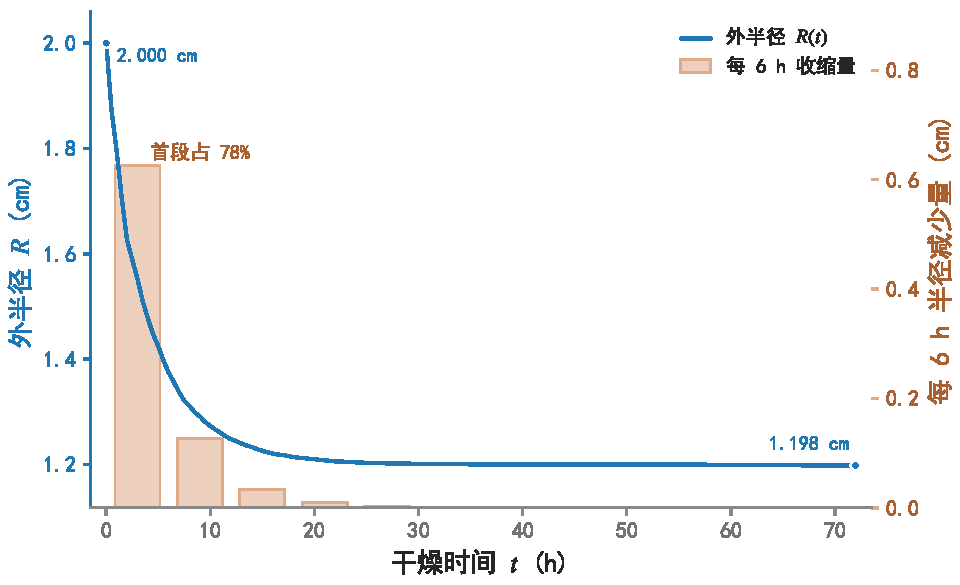
\includegraphics[width=0.9\textwidth,height=0.8\textheight,keepaspectratio]{../figures/fig_shrinkage_curve.pdf}
  \caption{药材半径收缩曲线}
  \label{fig:shrinkage_curve}
\end{figure}

收缩几乎全部发生在烘干初期（图~\ref{fig:shrinkage_curve}~给出附件 2 全部
$145$ 个点的半径时程与每 $6$ h 的收缩增量）。半径由 $2.000$ cm 单调降到 $1.198$ cm，
横截面积仅剩初始的 $35.88\%$。收缩的时间分布极不均匀：
前 $6$ h 内半径就下降 $0.626$ cm，占全程总收缩量的 $78.1\%$；
到 $12$ h 累计完成 $93.8\%$；$36$ h 之后半径几乎冻结在 $1.200$ cm。

这一形态决定了收缩的作用不容小视。前 $6$ h 正是含水率梯度最陡、
传质最活跃的时段，扩散路程恰在最关键的阶段被缩短 $31.3\%$。
由式~\eqref{eq:mass_s}，半径由 $2.000$ cm 降到 $1.374$ cm 使系数 $4/R^2$
放大到 $2.12$ 倍，收缩到最小半径 $1.198$ cm 时更达 $2.79$ 倍，
等效于扩散被显著加速。

\fi
\subsection{结果}

按 $N=160$、$\Delta t=1$ s 推进到第 $183\,900$ 步（即 $51.0833$ h）时判据首次满足，
与问题三同法插值得

\begin{equation}
t_{\mathrm{dry}}=51.0711~\text{h}=2.1280~\text{d}.
\label{eq:tdry_q4}
\end{equation}

末输出步 $\max_rC=0.149977$ 已低于阈值、前一步 $0.150008$ 仍高于阈值，
确为首次穿越；全程守恒残差 $1.547\times10^{-10}$。
网格无关性上，$N=48$、$112$、$160$ 分别给出 $51.042455$、$51.067066$、
$51.071110$ h，相邻相对差 $4.819\times10^{-4}$ 与 $7.919\times10^{-5}$，
末组远优于判据，对应图~\ref{fig:grid_convergence}~的第二条曲线。

与式~\eqref{eq:tdry_q3}~同理，式~\eqref{eq:tdry_q4}~也是条件式结论：
附件 1 实测只覆盖前 $4$ h，占本问总时长的 $7.8\%$，
其余 $92.2\%$ 的时间轴由平台均值常数延拓段提供边界条件，
第~\ref{sec:validation}~节给出的 $\pm0.5$ °C 扰动对应约 $\mp1.6\%$ 的时长变化。
问题四还多一重不确定度来源：半径时程是最灵敏的输入，
半径弹性达 $1.810$，故式~\eqref{eq:tdry_q4}~应理解为
“在恒温平台条件持续保持、且附件 2 半径数据准确的前提下”的烘干时长。

\begin{figure}[!htbp]
  \centering
  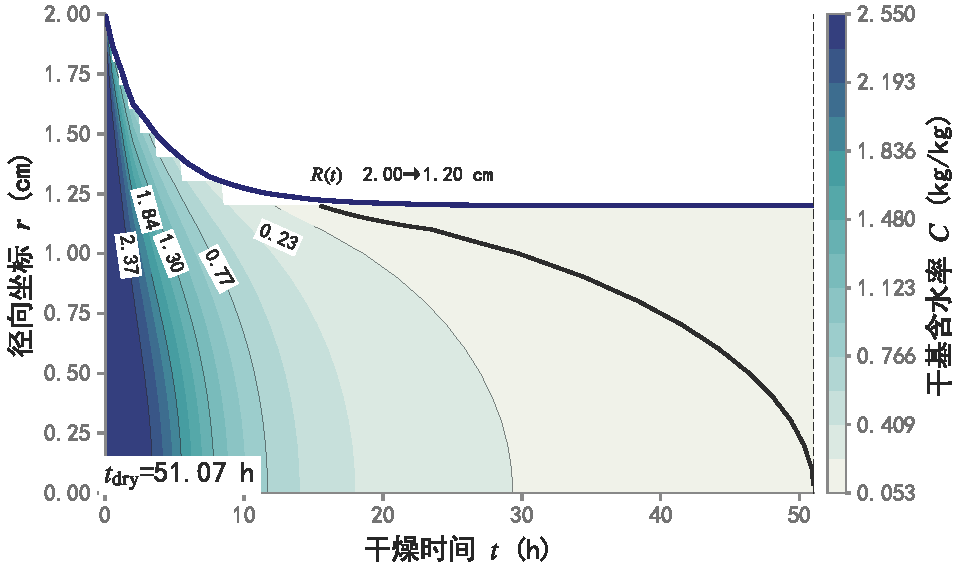
\includegraphics[width=0.74\textwidth,height=0.42\textheight,keepaspectratio]{../figures/fig_q4_field_C_moving.pdf}
  \caption{问题四移动边界含水率场}
  \label{fig:q4_field_C_moving}
\end{figure}

移动边界在前 $6$ h 迅速内收、随后趋于水平，
而含水率等值线始终与边界保持相似的排布
（图~\ref{fig:q4_field_C_moving}~在含水率场上叠加 $R(t)$ 曲线，域外区域留白）。
等值线与边界的这种相似排布，是仿射收缩假设下每个 $s$ 值
标记同一批干物质的直观体现。留白区域并非缺失数据，
而是该时刻药材已经收缩到那个半径之内，物理上不存在的位置不做插值编造。

\begin{table}[H]
  \centering
  \caption{问题四烘干过程的水分浓度（kg/kg）}
  \label{tab:q4_C}
  \setlength{\tabcolsep}{4pt}
  \begin{tabular}{ccccccc}
  \toprule
  时间 (h) & $R(t)$ (cm) & $r=0$ cm & $r=0.5$ cm & $r=1.0$ cm & 药材表面 & $\bar C$ \\
  \midrule
  6  & 1.3740 & 1.7195 & 1.5376 & 1.0226 & 0.4208 & 1.0652 \\
  12 & 1.2480 & 0.7375 & 0.6545 & 0.4082 & 0.1669 & 0.4760 \\
  18 & 1.2140 & 0.4086 & 0.3686 & 0.2397 & 0.0892 & 0.2803 \\
  24 & 1.2040 & 0.2850 & 0.2610 & 0.1789 & 0.0673 & 0.2054 \\
  30 & 1.2010 & 0.2263 & 0.2093 & 0.1492 & 0.0595 & 0.1685 \\
  36 & 1.2000 & 0.1928 & 0.1796 & 0.1316 & 0.0559 & 0.1469 \\
  42 & 1.2000 & 0.1712 & 0.1603 & 0.1199 & 0.0541 & 0.1327 \\
  48 & 1.2000 & 0.1561 & 0.1468 & 0.1115 & 0.0530 & 0.1225 \\
  烘干结束 51.0711 & 1.2000 & 0.1500 & 0.1413 & 0.1081 & 0.0526 & 0.1184 \\
  \bottomrule
  \end{tabular}
\end{table}

表~\ref{tab:q4_C}~的列式与问题三不同，末列为药材表面处的数值，
这是题面明确要求的格式，也是收缩问题下唯一自洽的写法：
$t\ge6$ h 时 $R(t)<1.5$ cm，$r=1.5$ cm 与 $r=2.0$ cm 两个位置
已经在药材之外，硬套问题三的固定半径列会得到没有物理意义的数值。
每隔 $60$ s、每隔 $0.1$ cm 的完整结果见 \verb|result4.xlsx|，
共 $3065$ 行 $\times$ $23$ 列：按第~\ref{sec:p1}~节说明的列数计法，
即一列时间标签加 $0$ 至 $2.0$ cm 共 $21$ 个半径列，再加“药材表面”末列。
超出当时 $R(t)$ 的位置留空，共 $23\,157$ 个空单元，
占 $21$ 个半径列的 $36.0\%$，不做域外插值。
若只关心全程始终有值的部分，$0$ 至 $1.1$ cm 的子集在整个烘干过程中
都位于药材内部，因为最小半径为 $1.198$ cm。

\subsection{消融实验：两个反向机制的分解}

式~\eqref{eq:tdry_q4}~比式~\eqref{eq:tdry_q3}~只短 $11.0\%$。
若就此结论“收缩影响有限”，会得到完全错误的物理图像，
因为问题四同时改动了物性与几何，而两者作用方向相反。
为把它们分开，本文按 $2\times2$ 设计做四次独立重算，
在 $N=112$、$\Delta t=1$ s 下统一比较。

\begin{table}[H]
  \centering
  \caption{物性与收缩的消融实验}
  \label{tab:ablation}
  \begin{tabular}{cccc}
  \toprule
  组合 & 物性闭合 & 几何 & $t_{\mathrm{dry}}$ (h) \\
  \midrule
  基准（问题三） & 附录 3 & $R\equiv R_0$ & 57.4040 \\
  仅换物性       & 附录 4 & $R\equiv R_0$ & 129.7587 \\
  仅加收缩       & 附录 3 & $R(t)$        & 25.2269 \\
  问题四（全）   & 附录 4 & $R(t)$        & 51.0671 \\
  \bottomrule
  \end{tabular}
\end{table}

两个主效应都很强且符号相反（表~\ref{tab:ablation}）。以下百分比一律以
该表首行的基准 $t_{\mathrm{base}}=57.4040$ h 为分母：
单换附录 4 使烘干时长增加 $126.0\%$（$+72.3547$ h），因为扩散系数小 $5.4$ 倍；
单加收缩使烘干时长减少 $56.1\%$（$-32.1771$ h），因为扩散路程被大幅缩短。
两者相加应为 $+40.1775$ h，而实测总变化只有 $-6.3370$ h，
交互项因此为

\begin{equation}
\Delta_{\mathrm{int}}
=t_{\mathrm{both}}-t_{\mathrm{base}}
-\left(t_{\mathrm{prop}}-t_{\mathrm{base}}\right)
-\left(t_{\mathrm{shrink}}-t_{\mathrm{base}}\right)
=-46.5145~\text{h}.
\label{eq:interaction}
\end{equation}

\iffalse
\begin{figure}[!htbp]
  \centering
  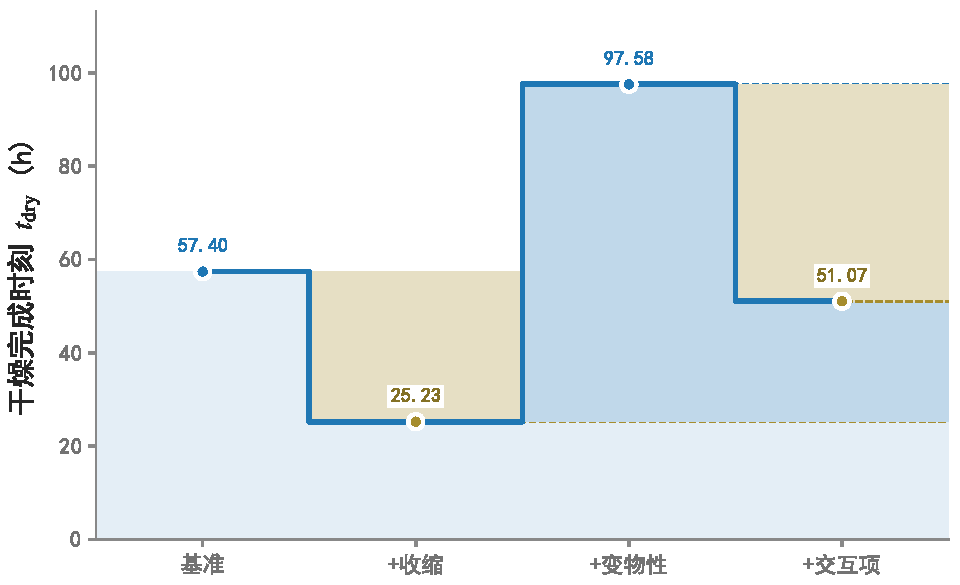
\includegraphics[width=0.9\textwidth,height=0.8\textheight,keepaspectratio]{../figures/fig_q4_ablation.pdf}
  \caption{收缩与物性的加性分解}
  \label{fig:q4_ablation}
\end{figure}

$+72.3547$ h 的物性效应、$-32.1771$ h 的收缩效应与 $-46.5145$ h 的交互项
合成最终的 $-6.3370$ h，瀑布图逐段给出这一累加过程
（图~\ref{fig:q4_ablation}）。交互项的量级与两个主效应相当，
说明两因素强耦合、不可线性叠加——收缩缩短路程的收益在扩散更慢的
附录 4 闭合下被进一步放大。

由此得到本问最重要的定性结论：收缩是本题最强的单一机制，
单独作用可把烘干时长压缩过半，只是在问题四中被附录 4 慢 $5.4$ 倍的扩散
大部分抵消，表面上才呈现为 $-11.0\%$ 的温和变化。
只报告净变化会掩盖这一事实。
\fi

\subsection{收缩数据与物性公式的一致性核查}

附件 2 的实测半径与附录 4 密度闭合在均质混合物假设下不相容：由半径反演的平均含水率自 $24$ h 起为负。本文因此以题目明确要求使用的实测半径为准；完整反演与讨论见附录 C。
\iffalse

附件 2 的实测半径与附录 4 的密度公式描述的是否同一件事，需要独立核查。
干质量线密度

\begin{equation}
\frac{M_s}{\pi L}=\frac{\rho_4(C_0)R_0^{2}}{1+C_0}=0.111493~\text{kg/m}
\label{eq:dry_linear}
\end{equation}

全程恒定。若认为整根药材的湿质量由附录 4 的 $\rho=760+90\bar C$ 描述，
则由实测半径可反演平均含水率：

\begin{equation}
\bar C_{\mathrm{vol}}(t)=\frac{0.111493-760R(t)^{2}}{90R(t)^{2}-0.111493}.
\label{eq:inversion}
\end{equation}

代入附件 2 的半径，$\bar C_{\mathrm{vol}}$ 在 $0$、$6$、$12$、$18$ h 处
分别为 $2.5500$、$0.3385$、$0.0706$、$0.0052$，自 $24$ h 起变为
$-0.0134$ 并继续下降到 $72$ h 的 $-0.0245$。含水率为负在物理上不可能，
说明这两处题设不能同时成立。

改用体积可加性闭合作对照，取 $\kappa=\rho_s/\rho_w=760/1000=0.7600$，
由 $V/V_0=(1+\kappa\bar C)/(1+\kappa C_0)$ 反演得 $\bar C(18~\text{h})=0.1086$，
而输运模型在同一时刻给出 $0.2803$，两者偏离 $61.3\%$。
两条路径在同一时刻相差如此之大，表明在“整根药材为均质两相混合物”这一
闭合假设下，附件 2 的收缩数据与附录 4 的物性公式不相容。
该结论依赖上述闭合假设，不能推广为两组数据本身必有一组错误。

这一矛盾无法在题设范围内消除，本文的处理是以附件 2 的实测半径为准，
理由有两条：题面明确要求“根据附件 2”确定烘干时长，实测数据的地位高于
由密度公式反推的间接量；且反演路径本身依赖“整根药材为均质两相混合物”
这一比输运模型更强的额外假设。同时必须承认这是问题四结果不确定度的
主要来源——第~\ref{sec:validation}~节的灵敏度分析显示 $R(t)$ 是全部参数中
最灵敏的一项，半径弹性达 $1.810$，故式~\eqref{eq:tdry_q4}~的可靠性
主要取决于附件 2 数据本身的可靠性。
\fi

\section{模型验证与敏感性摘要}
\label{sec:validation}

四问共用同一求解器，验证从独立解析解、离散收敛、守恒和结构性退化四个层面进行。问题一常物性温度方程的 Bessel--Duhamel 解与数值解最大偏差为 $5.224\times10^{-4}$ °C；问题三、四在 $N=160$ 时均满足相邻网格相对差不超过 $5\times10^{-4}$，而 $\Delta t$ 从 $4$ s 减至 $0.5$ s 仅使 $t_{\mathrm{dry}}$ 改变约 $3\times10^{-3}$ h。零输入、常空气解析、纯扩散守恒和收缩关闭四项退化检验均通过；四问守恒残差为 $10^{-11}\sim10^{-10}$。完整判据、逐档数据与图表见附录 C。

单因子重算表明，烘干时长的敏感性顺序为
\begin{equation}
R(t)\gg h_m>T_{\mathrm{air}}\gg W_{\mathrm{air}}\gg h.
\end{equation}
其中半径 $\pm5\%$ 引起约 $\pm9\%$ 的时长变化，中心差商弹性为 $1.810$；$h_m$ 减少 $20\%$ 使时长增加 $2.973\%$，而 $h$ 的双向扰动仅约 $\pm0.03\%$。这说明全过程由传质与几何尺度控制，未显式计入汽化潜热会影响表面温度估计，但不是时长的主导不确定度。两种烘干时长分别为 $2.3927$ d 和 $2.1280$ d，均位于题设给出的 $2$--$3$ d 先验区间内。

\begin{figure}[!htbp]
\centering
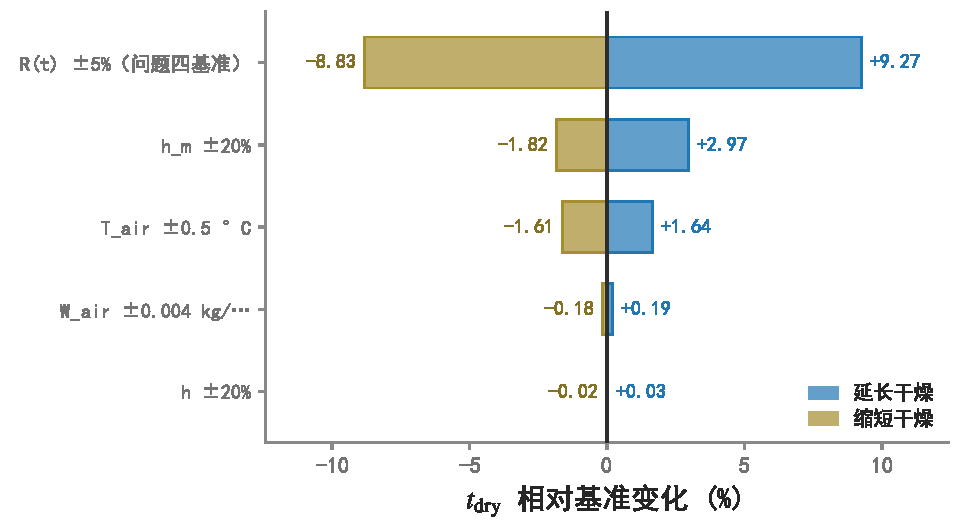
\includegraphics[width=.62\textwidth,height=.35\textheight,keepaspectratio]{../figures/fig_sensitivity_tornado.pdf}
\caption{单因子灵敏度排序}
\label{fig:sensitivity_tornado}
\end{figure}

\section{模型评价与推广}

\begin{table}[H]\centering\small
\caption{四问主结果汇总}\label{tab:main_results}
\setlength{\tabcolsep}{4pt}
\begin{tabular}{lllrr}\toprule
问题&物性闭合&几何&时间跨度或 $t_{\mathrm{dry}}$&结束时 $\max_rC$\\\midrule
问题一&附录 2 常物性&固定 $R$&1800 s&--\\
问题二&附录 3 变物性&固定 $R$&3 h&--\\
问题三&附录 3 变物性&固定 $R$&57.4247 h&0.1500\\
问题四&附录 4 变物性&$R(t)$ 收缩&51.0711 h&0.1500\\\bottomrule
\end{tabular}\end{table}

本文的四问不是四套孤立模型，而是同一热质输运框架在物性闭合与几何条件上的递进。其关键设计包括：以干质量拉格朗日坐标 $s=(r/R(t))^2$ 固定移动域；以节点中心有限体积直接装配 Robin 边界；用 Bessel--Duhamel 解析解独立校验常物性温度场；以 $2\times2$ 消融实验分离物性、收缩及其交互。后者表明，问题四相对问题三的净时长变化不能直接归因于收缩：物性效应为 $+126.0\%$、收缩效应为 $-56.1\%$，交互项为 $-46.5145$ h。

模型的局限也明确：一维径向近似忽略端面输运，故时长偏向保守；未显式计入汽化潜热和吸附等温线，温度场尤其是表面温度可能偏高；问题三、四中约 $93\%$ 时间轴依赖末段恒温平台延拓；附件 2 半径与附录 4 密度闭合在均质假设下不相容。因此，结果应理解为题给边界、实测半径和指定物性闭合共同条件下的预测。

若补充潜热、吸附等温线或更完整的几何数据，现有求解器可分别扩展为真正热质边界耦合、由含水率驱动的收缩本构和二维轴对称模型；若研究工艺优化，则可将本正问题嵌入能耗--时长外层搜索，优先调控半径尺度相关的装载方式与传质条件。


% === 参考文献 ===
% AI 工具使用声明由 build_ai_disclosure.py 自动插入到本环境之前。
% === AI 工具使用声明（自动插入）===
\section*{AI 工具使用声明}
本参赛队在竞赛过程中使用了 AI 工具，用于代码调试、论文撰写辅助与语言润色。
模型建立、参数设定、数值求解和结论形成均由参赛队独立完成；详细使用情况、人工修改及核验记录见支撑材料。

\begin{thebibliography}{99}
\bibitem{khallaf2022herbs}
KHALLAF A E M, EL-SEBAII A A. Review on drying of the medicinal plants (herbs)
using solar energy applications[J]. Heat and Mass Transfer, 2022.
DOI: 10.1007/s00231-022-03191-5.

\bibitem{le2025acori}
LE Y N, ZHANG J L, ZHONG L Y, et al. Drying kinetics and characteristics of
Acori Tatarinowii Rhizoma under hot air thin-layer drying at different
temperatures[J]. Research Square Preprint, 2025.
DOI: 10.21203/rs.3.rs-5772980/v1.

\bibitem{adrover2019twod}
ADROVER A, BRASIELLO A. A moving boundary model for food isothermal drying and
shrinkage: One-dimensional versus two-dimensional approaches[J]. Journal of
Food Process Engineering, 2019. DOI: 10.1111/jfpe.13178.

\bibitem{luikov1966capillary}
LUIKOV A V. Heat and mass transfer in capillary-porous bodies[M]//Heat and Mass
Transfer in Capillary-Porous Bodies. Oxford: Pergamon Press, 1966.
DOI: 10.1016/b978-1-4832-0065-1.50010-6.

\bibitem{onwude2016pumpkin}
ONWUDE D I, HASHIM N, JANIUS R, et al. Modelling effective moisture diffusivity
of pumpkin (Cucurbita moschata) slices under convective hot air drying
condition[J]. International Journal of Food Engineering, 2016.
DOI: 10.1515/ijfe-2015-0382.

\bibitem{dedic2002wood}
DEDIC A D. Modelling of coupled heat and mass transfer during convective drying
of wood[J]. Drying Technology, 2002. DOI: 10.1081/drt-120004320.

\bibitem{adrover2019general}
ADROVER A, BRASIELLO A, PONSO G. A moving boundary model for food isothermal
drying and shrinkage: General setting[J]. Journal of Food Engineering, 2019.
DOI: 10.1016/j.jfoodeng.2018.09.018.

\bibitem{krokida1998shrinkage}
KROKIDA M K, KARATHANOS V T, MAROULIS Z B. Effect of freeze-drying conditions
on shrinkage and porosity of dehydrated agricultural products[J]. Journal of
Food Engineering, 1998. DOI: 10.1016/s0260-8774(98)00031-4.

\bibitem{luikov1966surface}
LUIKOV A V. Heat and mass transfer of a solid body with the surrounding
medium[M]//Heat and Mass Transfer in Capillary-Porous Bodies. Oxford: Pergamon
Press, 1966. DOI: 10.1016/b978-1-4832-0065-1.50008-8.

\bibitem{adrover2019shortcut}
ADROVER A, BRASIELLO A, PONSO G. A moving boundary model for food isothermal
drying and shrinkage: A shortcut numerical method for estimating the shrinkage
factor[J]. Journal of Food Engineering, 2019.
DOI: 10.1016/j.jfoodeng.2018.09.030.

\bibitem{zhang2022fv}
ZHANG B Y, FU H F, LIANG X T, et al. An efficient second-order finite volume
ADI method for nonlinear three-dimensional space-fractional reaction-diffusion
equations[J]. Advances in Applied Mathematics and Mechanics, 2022.
DOI: 10.4208/aamm.oa-2021-0153.

\bibitem{cruz2019implicit}
CRUZ-RODRIGUEZ R C, SKIBA Y N, FILATOV D M. An implicit direct unconditionally
stable numerical algorithm for the solution of advection-diffusion equation on
a sphere[J]. Applied Numerical Mathematics, 2019.
DOI: 10.1016/j.apnum.2019.02.006.

\bibitem{guellal2009cylinder}
GUELLAL M, SADAT H, PRAX C. A simple model for transient heat conduction in an
infinite cylinder with convective boundary conditions[J]. Journal of Heat
Transfer, 2009. DOI: 10.1115/1.3082428.

\bibitem{zare2018analytic}
ZARE M, KARDAN F. Analytical solution based on a new series along with the
numeric solution of the non-homogeneous transient heat conduction equation, in
hollow cylinder under general mixed boundary conditions[J]. American Journal of
Engineering and Applied Sciences, 2018. DOI: 10.3844/ajeassp.2018.538.547.

\bibitem{singh2018potato}
SINGH D, SINGH P, TALUKDAR P. Coupled fluid flow and simultaneous heat and mass
transfer model for convective drying of potato[C]//Proceedings of the 24th
National and 2nd International ISHMT-ASTFE Heat and Mass Transfer Conference.
2018. DOI: 10.1615/ihmtc-2017.1570.

\bibitem{chigbo2024thinlayer}
CHIGBO K S, LINUS-CHIBUEZEH A, MOUFUNANYA U F, et al. Mathematical modeling of
the effects of thickness and temperature on thin-layer drying kinetics of
oven-dried cooking bananas slices[J]. Food Production, Processing and
Nutrition, 2024. DOI: 10.1186/s43014-024-00233-9.

\bibitem{rodriguez2014thyme}
RODRIGUEZ J, CLEMENTE G, SANJUAN N, et al. Modelling drying kinetics of thyme
(Thymus vulgaris L.): Theoretical and empirical models, and neural networks[J].
Food Science and Technology International, 2014.
DOI: 10.1177/1082013212469614.

\bibitem{benseddik2023inverse}
BENSEDDIK A, BENSAHA H, LALMI D, et al. An inverse method for determining the
instantaneous diffusion coefficient of pumpkin slices during drying process[J].
Latin American Applied Research, 2023. DOI: 10.52292/j.laar.2023.976.

\end{thebibliography}
\label{mh:body-end}

% === 附录 ===
\begin{appendices}
\section{程序结构与交付文件说明}

本文的全部计算由一套 Python 程序完成，运行 \verb|code/main.py| 即可依次复现
四问结果与全部检验。程序分工如下：\verb|params.py| 集中存放题给参数与三套
物性闭合；\verb|utils.py| 提供附件插值、节点中心有限体积装配与三对角求解；
\verb|problem1.py| 至 \verb|problem4.py| 分别对应四问，其中 \verb|problem1.py|
另含 Bessel--Duhamel 解析解；\verb|problem3_sens.py| 执行单因子灵敏度重算；
\verb|data_check.py| 与 \verb|sanity_check.py| 完成附件读入核对与结构性退化检验；
\verb|constraint_audit.py| 从落盘结果重算全部数值约束。
依赖版本记录在 \verb|code/requirements.txt|。

\subsection*{支撑材料文件清单}
支撑材料以 \verb|.zip| 压缩包提交，解压后保持以下目录结构：
\begin{itemize}
  \item \verb|code/|：\verb|main.py|、\verb|params.py|、\verb|utils.py|、
  \verb|problem1.py| 至 \verb|problem4.py|、\verb|problem3_sens.py|、
  \verb|data_check.py|、\verb|sanity_check.py|、\verb|constraint_audit.py| 和
  \verb|requirements.txt|；
  \item \verb|figures/|：正文 24 张图的 PDF 文件、对应绘图脚本、表格源文件及流程图源文件；
  \item \verb|user_data/|：\verb|附件1.xlsx|、\verb|附件2.xlsx| 与
  \verb|result1.xlsx| 至 \verb|result4.xlsx|；
  \item 根目录文件：\verb|PROBLEM_FACTS.json|、\verb|DATA_PROFILE.json|、
  \verb|requirements.txt|、\verb|README.txt| 和 \verb|AI工具使用详情.pdf|。
\end{itemize}
其中，\verb|README.txt| 说明运行环境与入口；两份 \verb|.json| 文件为当前程序读取的
参数口径和数据行数配置，须与源代码一并保留。

交付的四个结果文件为 \verb|result1.xlsx| 至 \verb|result4.xlsx|，
依次对应四问，规模依次为
$1800\times22$（温度、水分浓度两张工作表）、$10800\times22$（两张工作表）、
$3446\times22$ 与 $3065\times23$，列数均按含时间列的表头长度计，
全部数值保留四位小数。

有一处交付文件之间的差异需要说明：问题二与问题三求解的是同一个初边值问题，
但制表精度要求不同，前者取 $\Delta t=0.5$ s、后者取 $1$ s。
在两文件重叠的 $60$ 至 $10800$ s 共 $180$ 个同列时刻上逐点比对，
最大绝对差为 $2.0\times10^{-4}$，出现在 $t=60$ s，
差值不小于 $10^{-4}$ 的时刻有 $162$ 个。因两文件均保留四位小数，
该差异在末位上可见。其量级远小于时间步无关性给出的模型不确定度——
$\Delta t$ 由 $4$ s 收到 $0.5$ s 只使 $t_{\mathrm{dry}}$ 改变
$3.0\times10^{-3}$ h，故不影响任何结论。

\section{核心程序源代码}

\lstset{basicstyle=\scriptsize\ttfamily,breaklines=true,columns=fullflexible,keepspaces=true,numbers=left,numberstyle=\tiny\color{gray}}

\subsection{参数与物性闭合 params.py}
\lstinputlisting[language=Python]{../code/params.py}

\subsection{插值、离散与求解内核 utils.py}
\lstinputlisting[language=Python]{../code/utils.py}

\subsection{问题一与解析校验 problem1.py}
\lstinputlisting[language=Python]{../code/problem1.py}

\subsection{问题二 problem2.py}
\lstinputlisting[language=Python]{../code/problem2.py}

\subsection{问题三 problem3.py}
\lstinputlisting[language=Python]{../code/problem3.py}

\subsection{问题四与消融实验 problem4.py}
\lstinputlisting[language=Python]{../code/problem4.py}

\subsection{灵敏度重算 problem3\_sens.py}
\lstinputlisting[language=Python]{../code/problem3_sens.py}

\subsection{结构性退化检验 sanity\_check.py}
\lstinputlisting[language=Python]{../code/sanity_check.py}

\subsection{主入口 main.py}
\lstinputlisting[language=Python]{../code/main.py}

\section{扩展模型推导与结果图}

本附录保留正文中为控制篇幅而不逐项展开的推导、对照图与补充说明；正文中的结论、控制方程、题设要求表格及关键数值均不依赖本附录才能理解。

\subsection{节点中心有限体积离散}
在 $s\in[0,1]$ 上取节点 $s_i=i\Delta s$。以水分方程为例，界面通量为
\begin{equation}
G_{i+1/2}=s_{i+1/2}D_{i+1/2}\frac{C_{i+1}-C_i}{\Delta s},\qquad D_{i+1/2}=\tfrac12(D_i+D_{i+1}).
\end{equation}
内部、轴心和表面半控制体分别满足
\begin{align}
\Delta s\frac{\mathrm dC_i}{\mathrm dt}&=\frac4{R^2}(G_{i+1/2}-G_{i-1/2}),\\
\frac{\Delta s}{2}\frac{\mathrm dC_0}{\mathrm dt}&=\frac4{R^2}G_{1/2},\\
\frac{\Delta s}{2}\frac{\mathrm dC_N}{\mathrm dt}&=-\frac4{R^2}G_{N-1/2}-\frac{2h_m}{R}(C_N-W_{\mathrm{air}}).
\end{align}
温度方程仅将 $D,h_m,W_{\mathrm{air}}$ 依次替换为 $k,h,T_{\mathrm{air}}$，并保留 $\rho c_p$。节点中心半控制体使 Robin 通量直接装配，无需虚拟节点。

\begin{figure}[H]\centering
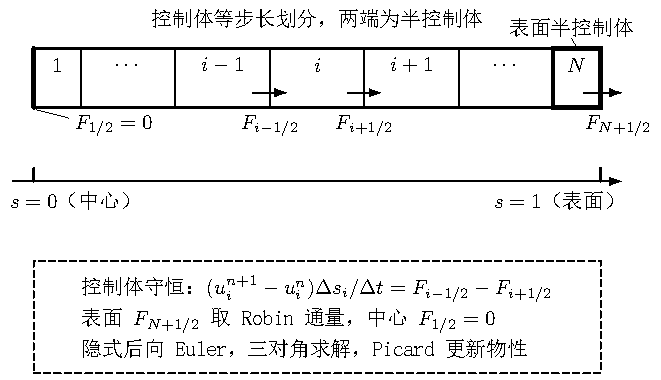
\includegraphics[width=.58\textwidth]{../figures/tikz_fv_stencil.pdf}
\caption{节点中心有限体积控制体与通量}\end{figure}

\subsection{问题一的扩展图与解析校验}
常物性温度方程的 Robin 特征函数为 $X_n=J_0(\zeta_n r/R_0)$，其中
\begin{equation}
\zeta_nJ_1(\zeta_n)=\mathrm{Bi}J_0(\zeta_n),\qquad \lambda_n=\alpha\zeta_n^2/R_0^2.
\end{equation}
令 $\theta=T-T_{\mathrm{air}}(t)$，则 $\dot b_n=-\lambda_nb_n-A_n\dot T_{\mathrm{air}}$；附件分段线性时逐段精确积分。该独立解与数值解的最大温度偏差为 $5.224\times10^{-4}$ °C。
\begin{figure}[H]\centering
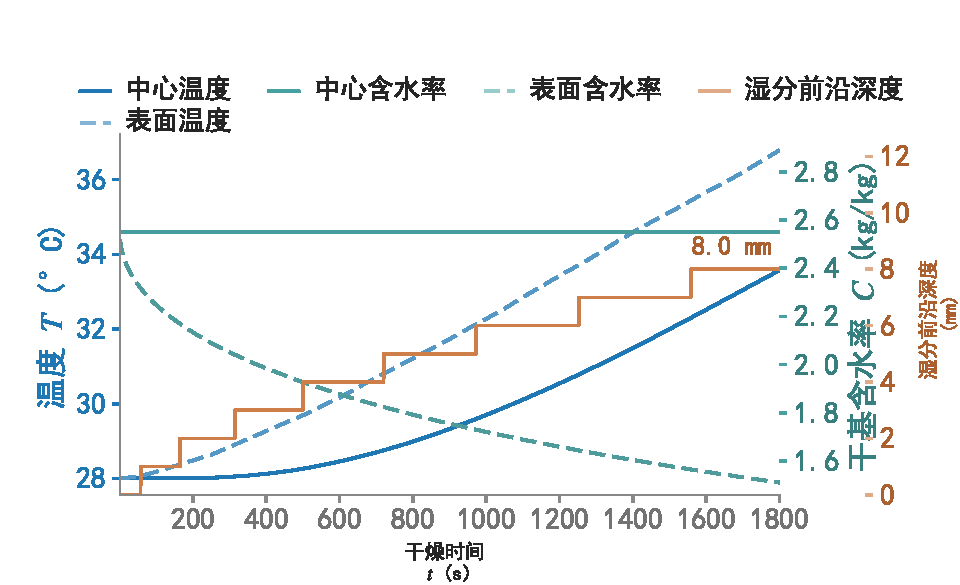
\includegraphics[width=.72\textwidth]{../figures/fig_q1_penetration.pdf}
\caption{问题一热湿推进对比}\end{figure}
\begin{figure}[H]\centering
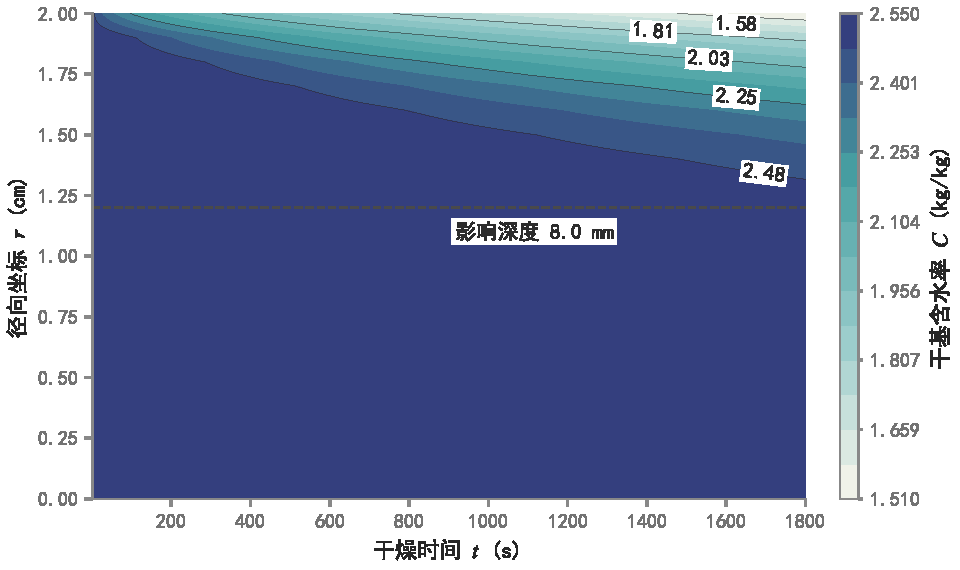
\includegraphics[width=.72\textwidth]{../figures/fig_q1_field_C.pdf}
\caption{问题一含水率场分布}\end{figure}
\begin{figure}[H]\centering
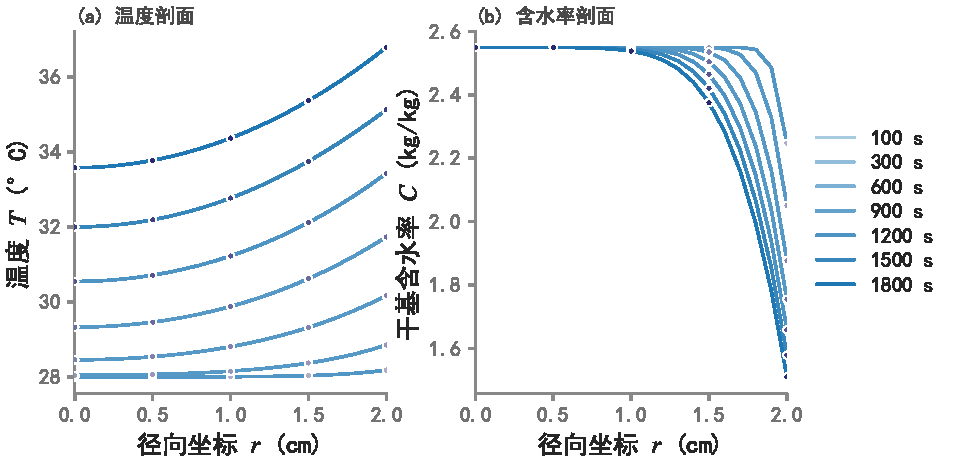
\includegraphics[width=.72\textwidth]{../figures/fig_q1_profiles.pdf}
\caption{问题一径向剖面族}\end{figure}
\begin{figure}[H]\centering
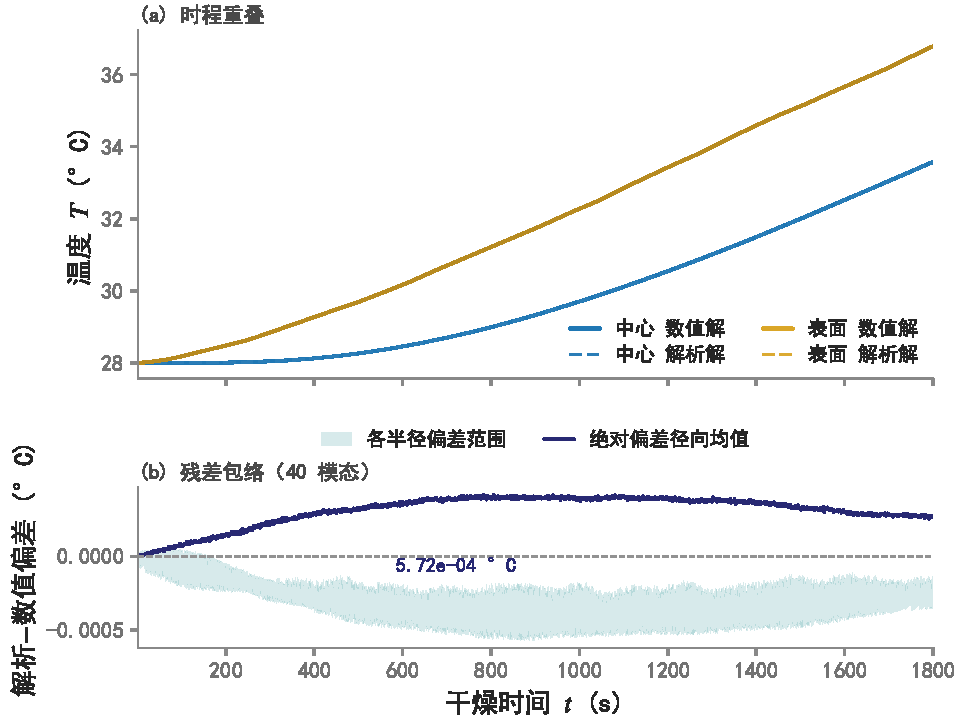
\includegraphics[width=.72\textwidth]{../figures/fig_q1_analytic_val.pdf}
\caption{问题一解析解与数值解完整对比}\label{fig:q1_analytic_val}\end{figure}

\subsection{问题二的扩展结果}
\begin{figure}[H]\centering
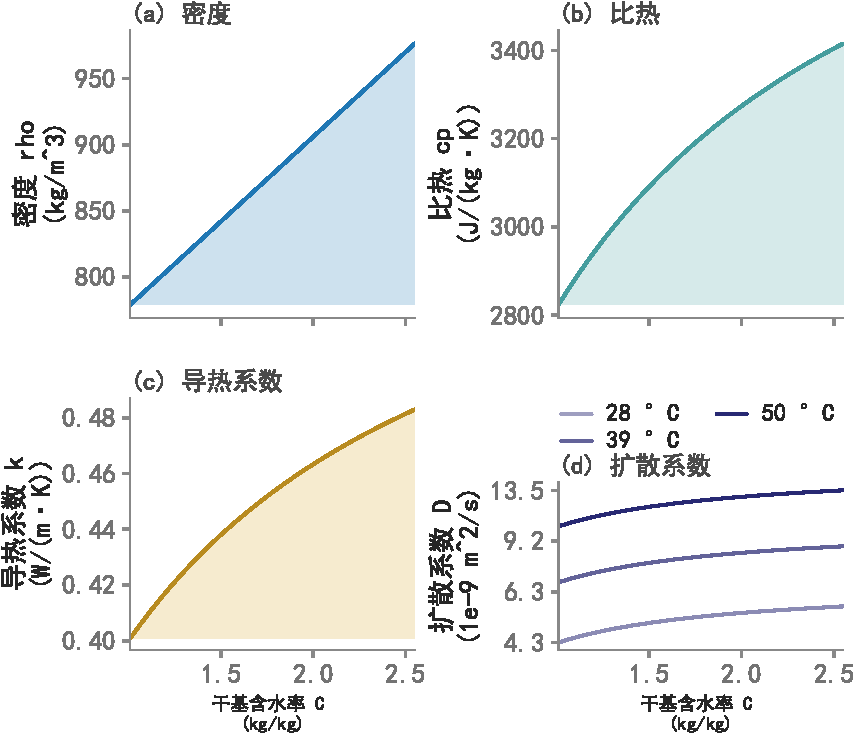
\includegraphics[width=.72\textwidth]{../figures/fig_q2_props_evolution.pdf}
\caption{附录三物性随含水率变化}\label{fig:q2_props_evolution}\end{figure}
\begin{figure}[H]\centering
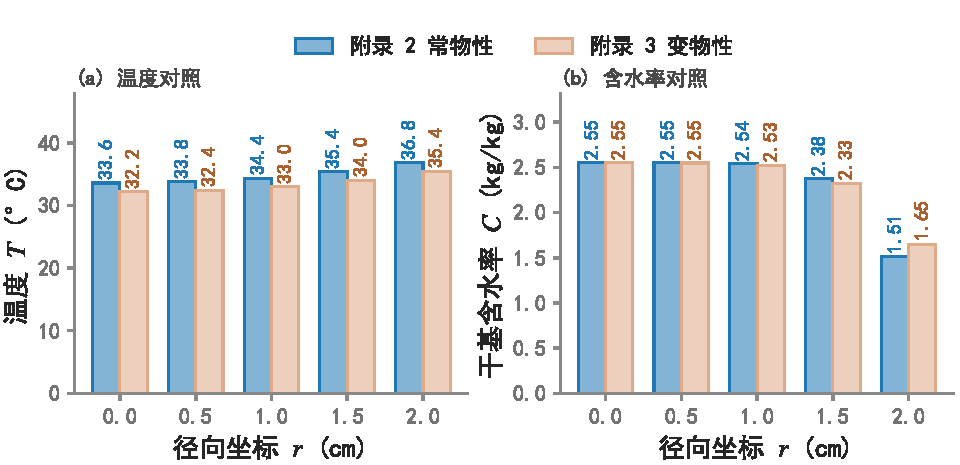
\includegraphics[width=.72\textwidth]{../figures/fig_q1q2_contrast.pdf}
\caption{常物性与变物性在 $1800$ s 的对照}\end{figure}
\begin{figure}[H]\centering
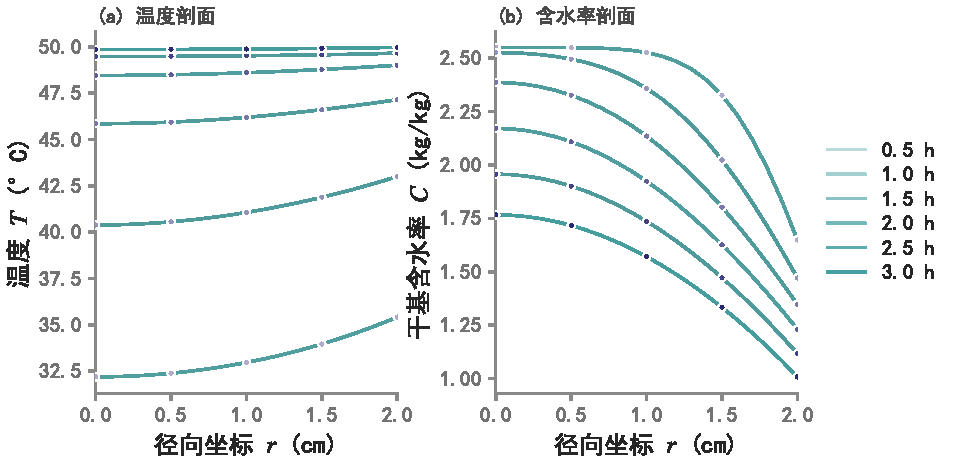
\includegraphics[width=.72\textwidth]{../figures/fig_q2_profiles.pdf}
\caption{问题二径向剖面族}\end{figure}

\subsection{问题四的扩展结果}
\begin{figure}[H]\centering
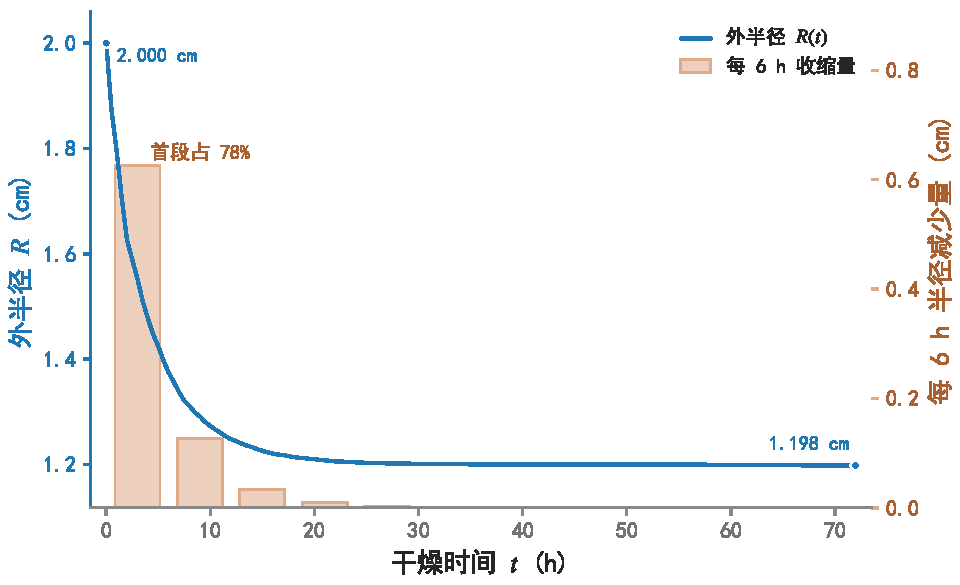
\includegraphics[width=.68\textwidth]{../figures/fig_shrinkage_curve.pdf}
\caption{药材半径收缩曲线}\end{figure}
\begin{figure}[H]\centering
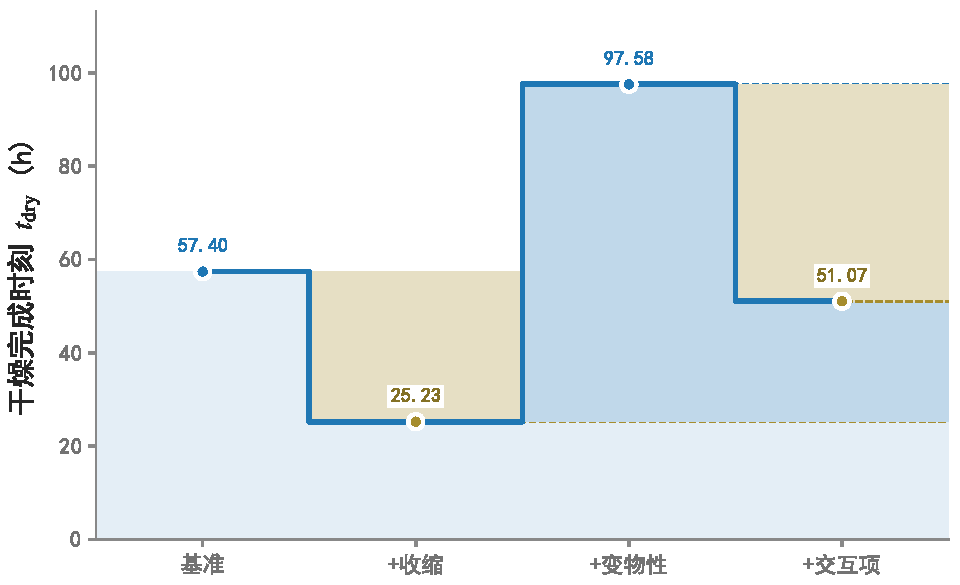
\includegraphics[width=.72\textwidth]{../figures/fig_q4_ablation.pdf}
\caption{收缩与物性的加性分解}\end{figure}

\section{数值验证、收敛性与灵敏度完整结果}
\begin{figure}[H]\centering
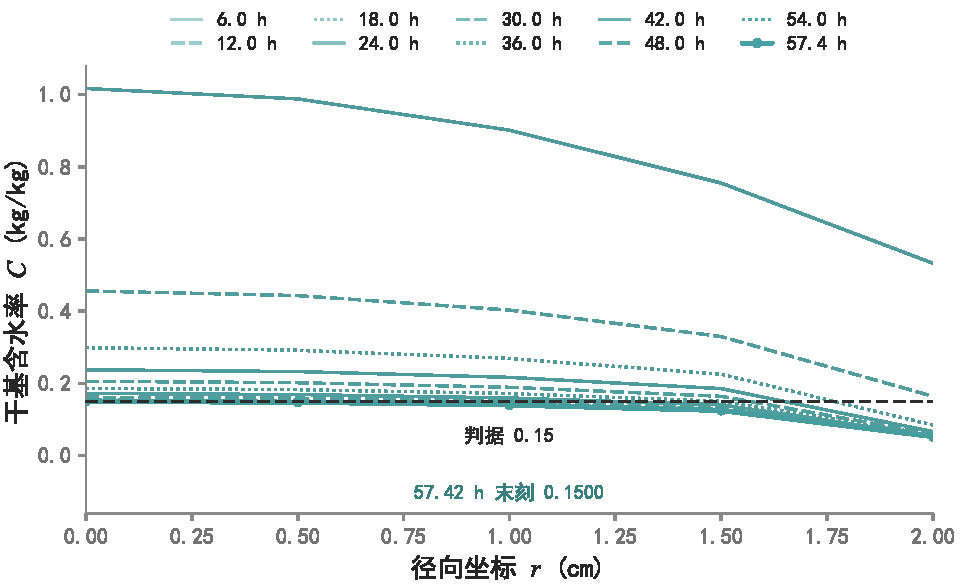
\includegraphics[width=.72\textwidth]{../figures/fig_q3_profiles_6h.pdf}
\caption{问题三每六小时径向剖面}\end{figure}
\subsection{网格和时间步收敛}
\begin{figure}[H]\centering
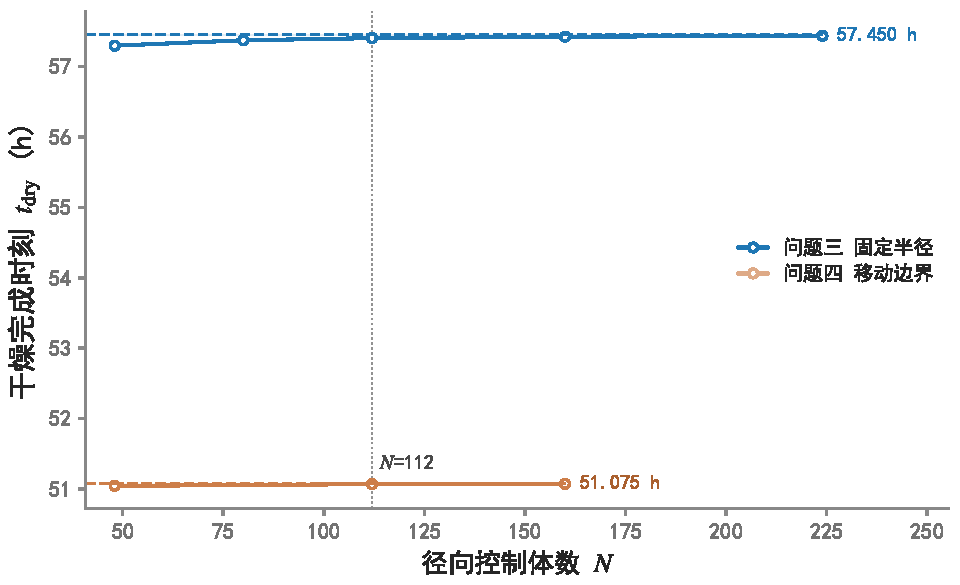
\includegraphics[width=.68\textwidth]{../figures/fig_grid_convergence.pdf}
\caption{问题三、四网格收敛轨迹}\label{fig:grid_convergence}\end{figure}
\begin{table}[H]\centering\small\caption{问题三网格收敛性}\begin{tabular}{rrr}\toprule
$N$&$t_{\mathrm{dry}}$ (h)&相对前一档差(\%)\\\midrule
48&57.2968&--\\80&57.3738&0.1343\\112&57.4040&0.0527\\160&57.4247&0.0360\\224&57.4370&0.0214\\\bottomrule\end{tabular}\end{table}
\begin{table}[H]\centering\small\caption{问题三时间步收敛性}\begin{tabular}{rr}\toprule
$\Delta t$ (s)&$t_{\mathrm{dry}}$ (h)\\\midrule 4.0&57.4067\\2.0&57.4049\\1.0&57.4040\\0.5&57.4036\\\bottomrule\end{tabular}\end{table}

\subsection{结构性退化与守恒检验}
\begin{table}[H]\centering\small\caption{结构性退化检验结果}\begin{tabular}{lcc}\toprule
检验&判据&实测\\\midrule
零输入&$<10^{-10}$&$2.522\times10^{-13}$\\常空气解析&$<10^{-3}$&$2.165\times10^{-4}$\\纯扩散守恒&$<10^{-12}$&$1.132\times10^{-14}$\\收缩关闭&$<10^{-6}$&$0.000\times10^{0}$\\\bottomrule\end{tabular}\end{table}
\begin{table}[H]\centering\small\caption{各问干质量守恒残差}\begin{tabular}{lrr}\toprule
算例&步数&相对残差\\\midrule 问题一&7200&$4.218\times10^{-11}$\\问题二&21600&$2.139\times10^{-11}$\\问题三&206760&$3.425\times10^{-10}$\\问题四&183900&$1.547\times10^{-10}$\\\bottomrule\end{tabular}\end{table}

\subsection{单因子灵敏度完整结果}
\begin{figure}[H]\centering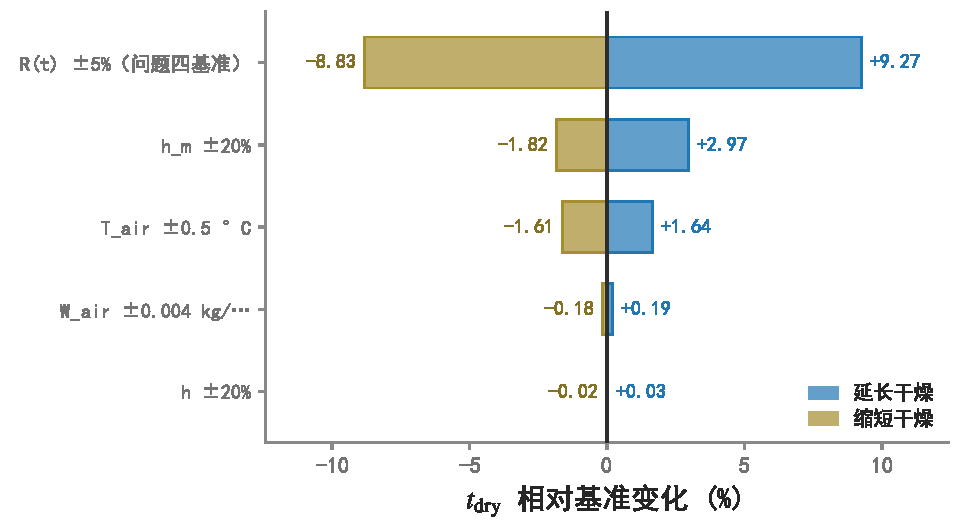
\includegraphics[width=.62\textwidth]{../figures/fig_sensitivity_tornado.pdf}\caption{单因子灵敏度排序}\end{figure}
完整结果表明 $R(t)\gg h_m>T_{\mathrm{air}}\gg W_{\mathrm{air}}\gg h$；半径 $\pm5\%$ 对应时长 $+9.273\%/-8.828\%$，其中心差商弹性为 $1.810$。

\end{appendices}

\end{document}
